\chapter{Resultados y discusi\'on}
\label{ch:resultadosRadio}

El objetivo de este cap\'itulo (y de la segunda parte de esta tesis) es estimar el desempe\~no  de un detector de antenas de radio a la hora de detectar neutrinos ES.
Para ello al igual que en Auger se calcular\'a la exposici\'on del detector, pero esta vez en una situaci\'on gen\'erica.
Se utilizar\'a lo estudiado en el capitulo \ref{ch:caracterizacionRadio} para definir el criterio de disparo global del detector hipot\'etico y se estimar\'an sus eficiencias de detecci\'on.
Todo lo anterior se realizar\'a utilizando distintas disposiciones espaciales de las antenas (topograf\'ias del detector), para encontrar una disposici\'on \'optima.
Finalmente, teniendo en cuenta todo lo anterior se comparar\'a su desempe\~no en relaci\'on a Auger y frente a la pr\'oxima generaci\'on de detectores de neutrinos ultra energ\'eticos.

\section{C\'alculo de la exposici\'on}
	
	Para calcular la exposici\'on en el detector se utiliz\'o una modificaci\'on de la ecuaci\'on \ref{eq:exp5ES} de la secci\'on \ref{sc:expoNu}, con la que se obtuvo la exposici\'on a neutrinos ES en Auger.
	Tales modificaciones fueron necesarias debido a que:
	\begin{enumerate}
	 \item Se incluy\'o la curvatura de la tierra en el c\'alculo de la exposici\'on.
	 \item Las eficiencias se calcularon en funci\'on de la energ\'ia visible.
	 \item Se considera un detector ideal, que no var\'ia a trav\'es del tiempo ni en su forma.
	\end{enumerate}
	%
	Estos tres puntos implican cambios en el t\'ermino de probabilidad, en las eficiencias y en las integrales que se deben realizar.
	Por este motivo las siguientes secciones se avocan a desarrollarlos en detalle.
	
% 	\begin{equation}
% 		\begin{aligned}
% 		{\cal E}_{ES}(E_\nu)\equiv2\pi\iiint\limits_{E_v~{\rm x_d}~\theta}P({\rm x_d},E_v|E_{\nu},\theta)~
% 		\left[~
% 		\iint\limits_{T~A}\epsilon({\rm x_d},E_v,A,\theta_D,T)~dA~dT
% 		\right]\\
% 		~\sen\theta_D d\theta_D~d{\rm x_d}~dE_v
% 		\end{aligned}
% 	 \label{eq:exp1ESRadio}
% 	\end{equation}
% 	%

	\subsection{Inclusi\'on de la curvatura de la tierra}
	El primer cambio en el c\'alculo es inducido por la inclusi\'on de la curvatura de la tierra en el modelo. 
	Esto resulta en que el \'angulo cenital con el que los neutrinos atraviezan la tierra, \te{}, difiere del observado sobre el detector \td{}, tal como se esquematiza en la figura \ref{fig:curveEarthSketch0}.
	%
	 \begin{figure}[ht!]
		\centering
		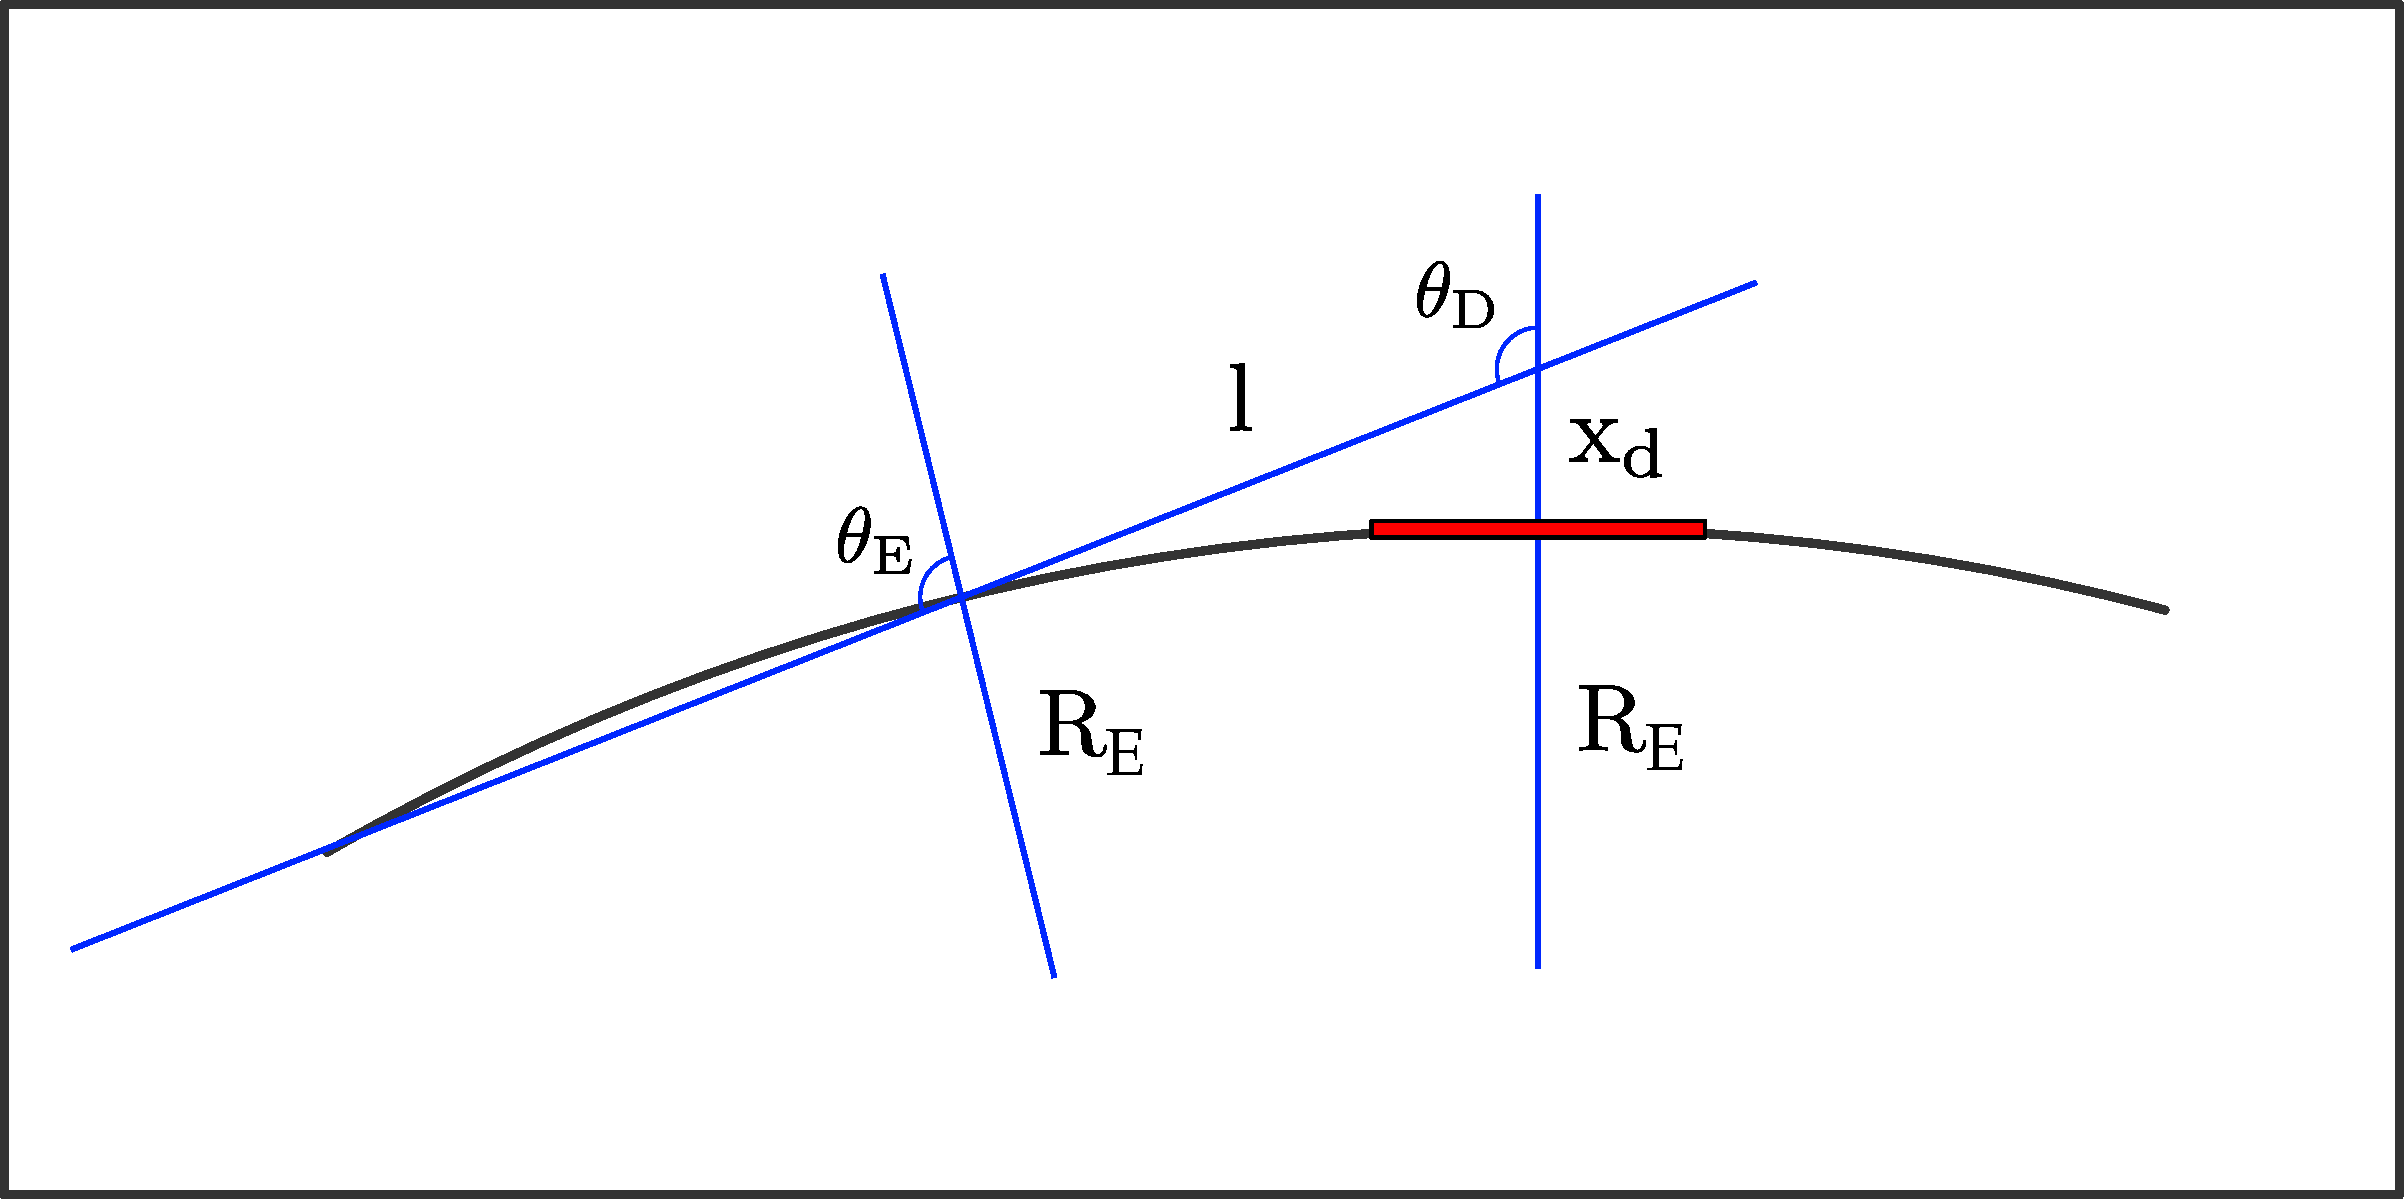
\includegraphics[width=0.8\textwidth]{./fig/appendix/curveEarthSketch.pdf}
		\caption{\label{fig:curveEarthSketch0}
		Esquema del cambio en el angulo sobre el detector y el utilizado para calcular las probabilidades de interacci\'on del neutrino en la tierra.
		}
	\end{figure}
	%
	Como consecuencia el c\'alculo se ve afectdo de dos maneras:
	\begin{enumerate}
	 \item Se modifican las probabilidades de decaimiento del \tauon{} en la atm\'osfera.
	 \item Para cada valor de \xd{} existe una zona de \'angulos cenitales sobre el detector prohibidos.
	\end{enumerate}
	
	\subsubsection{Cambio en las probabilidades de decaimiento en la atm\'osfera}
	Tal como se discuti\'o en la secci\'on \ref{sbsc:corrES}, el decaimiento del \tauon{} en la atm\'osfera se modela con una distribuci\'on exponencial, de forma:
	%
	\begin{equation}
		h({\rm x_d},(E_\tau,\theta_D))=
		\exp{\left(
		-\frac{l({\rm x_d},\theta_D)}{\lambda(E_\tau)}
		\right)}
		\frac{dl({\rm x_d})}{d{\rm x_d}}
		\frac{1}{\lambda(E_\tau)}
		\label{eq:decayTayRadio}
	\end{equation}
	%
	Entonces, si se tiene en cuenta la curvatura de la tierra, la expresi\'on de $l({\rm x_d},\theta_D)$ queda:
	%
	\begin{equation}
		\begin{array}{rcl}
		l({\rm x_d},\theta_D) & = & \dfrac{R_E^2-(R_E+{\rm x_d})^2}{R_E \cos \theta_E + (R_E+{\rm x_d}) \cos \theta_D}\\
		&&\\
		\end{array}
		\label{eq:l_curve0}
	\end{equation}
	donde $R_E$ es el radio de la tierra y:
	\begin{equation}
		\begin{array}{rcl}
		\cos \theta_E & = & - \left[ \dfrac{R_E^2 - (R_E+{\rm x_d})^2 (1-\cos^2 \theta_D)}{R_E^2} \right]^{\frac{1}{2}} \\ 
		\end{array}
		\label{eq:te_td0}
	\end{equation}
	%
	Luego, derivando \ref{eq:l_curve0} puede obtenerse anal\'iticamente la expresi\'on de $\frac{dl({\rm x_d})}{d{\rm x_d}}$:
	\begin{equation}
	\begin{aligned}
		\frac{dl({\rm x_d})}{d{\rm x_d}}
		=&-
		\frac{
		2(R_E+{\rm x_d})
		(R_E\cos{\theta_E}+(R_E+{\rm x_d}\cos{\theta_D}))
		}{
		(R_E\cos{\theta_E}+(R_E+{\rm x_d}\cos{\theta_D}))^2
		}\\
% 		\ & \\
		&-
		\frac{(R_E^2+(R_E+{\rm x_d})^2)(R_E\frac{d\cos{\theta_E}}{d{\rm x_d}}+\cos{\theta_D})
		}{
		(R_E\cos{\theta_E}+(R_E+{\rm x_d}\cos{\theta_D}))^2
		}
	\end{aligned}
	\end{equation}
	%
	con:
	\begin{equation}
	\frac{d\cos{\theta_E}}{d{\rm x_d}}
	=
	\frac{
	(R_E+{\rm x_d})
	(1-\cos^2\theta_D)
	}{\cos{\theta_E}R_E^2
	}
	\end{equation}
	%
	La derivaci\'on de estas ecuaciones puede encontrarse en el ap\'endice \ref{ap:tierraCurva} junto con un peque\~no an\'alisis de su impacto.
	
	\subsubsection{Regi\'on de \'angulos cenitales prohibidos}
	Por simple geometr\'ia, para cada valor de \xd{} aparecer\'a un \'angulo observado m\'inimo sobre el detector, $\theta_D^{cut}$, correspondiente al m\'inimo valor con el que los neutrinos pueden incidir sobre la tierra, $\theta_E=90^\circ$.
	Esta situaci\'on se bosqueja en la figura \ref{fig:curveEarthSketch_thCut0} y su valor puede calcularse anal\'iticamente (ver ap\'endice \ref{ap:tierraCurva}), mediante:
	\begin{equation}
	\cos \theta_D^{cut} = \left[ \frac{2 R_E {\rm x_d}+{\rm x_d}^2}{(R_E+{\rm x_d})^2} \right]^{\frac{1}{2}}
	\label{eq:tdc0}
	\end{equation}
	%
	\begin{figure}[ht!]
		\centering
		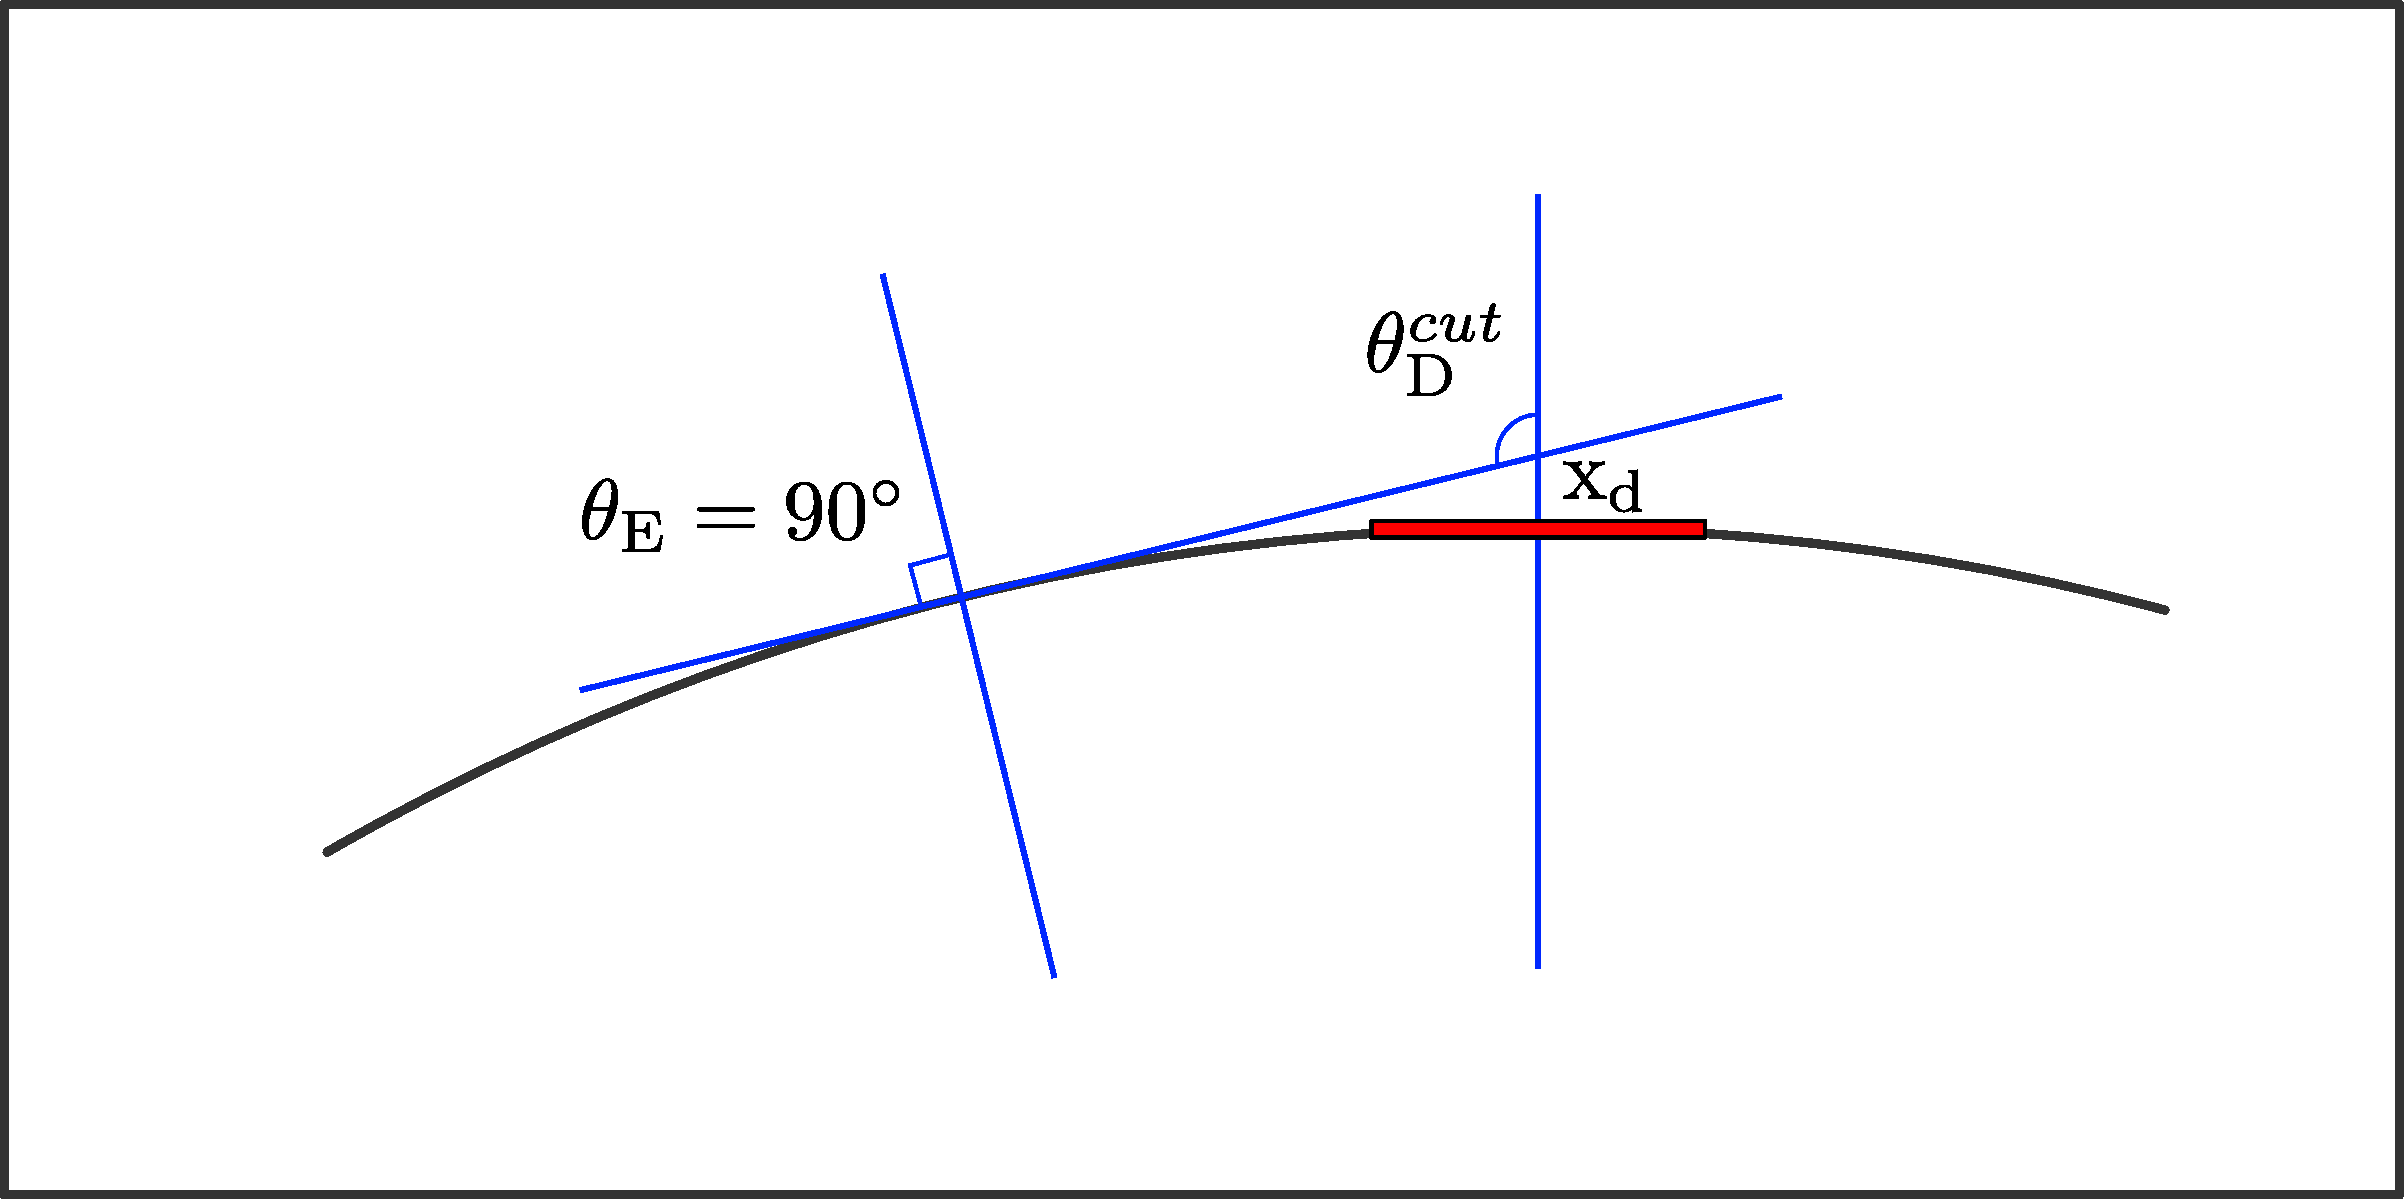
\includegraphics[width=0.8\textwidth]{./fig/appendix/curveEarthSketch_thCut.pdf}
		% curveEarthSketch.png: 2404x1199 pixel, 150dpi, 40.70x20.30 cm, bb=0 0 1154 575
		\caption{\label{fig:curveEarthSketch_thCut0}
		Dado \xd{} existe un valor m\'inimo de \td{}, $\theta_D^{cut}$, que corresponde a $\theta_E=90^\circ$.
		}
	\end{figure}
	%
	
	Entonces para cada \xd{} pueden calcularse los valores permitidos para \td{}, lo que se grafica en la figura \ref{fig:dx_thcut0}.
	\begin{figure}[ht!]
		\centering
		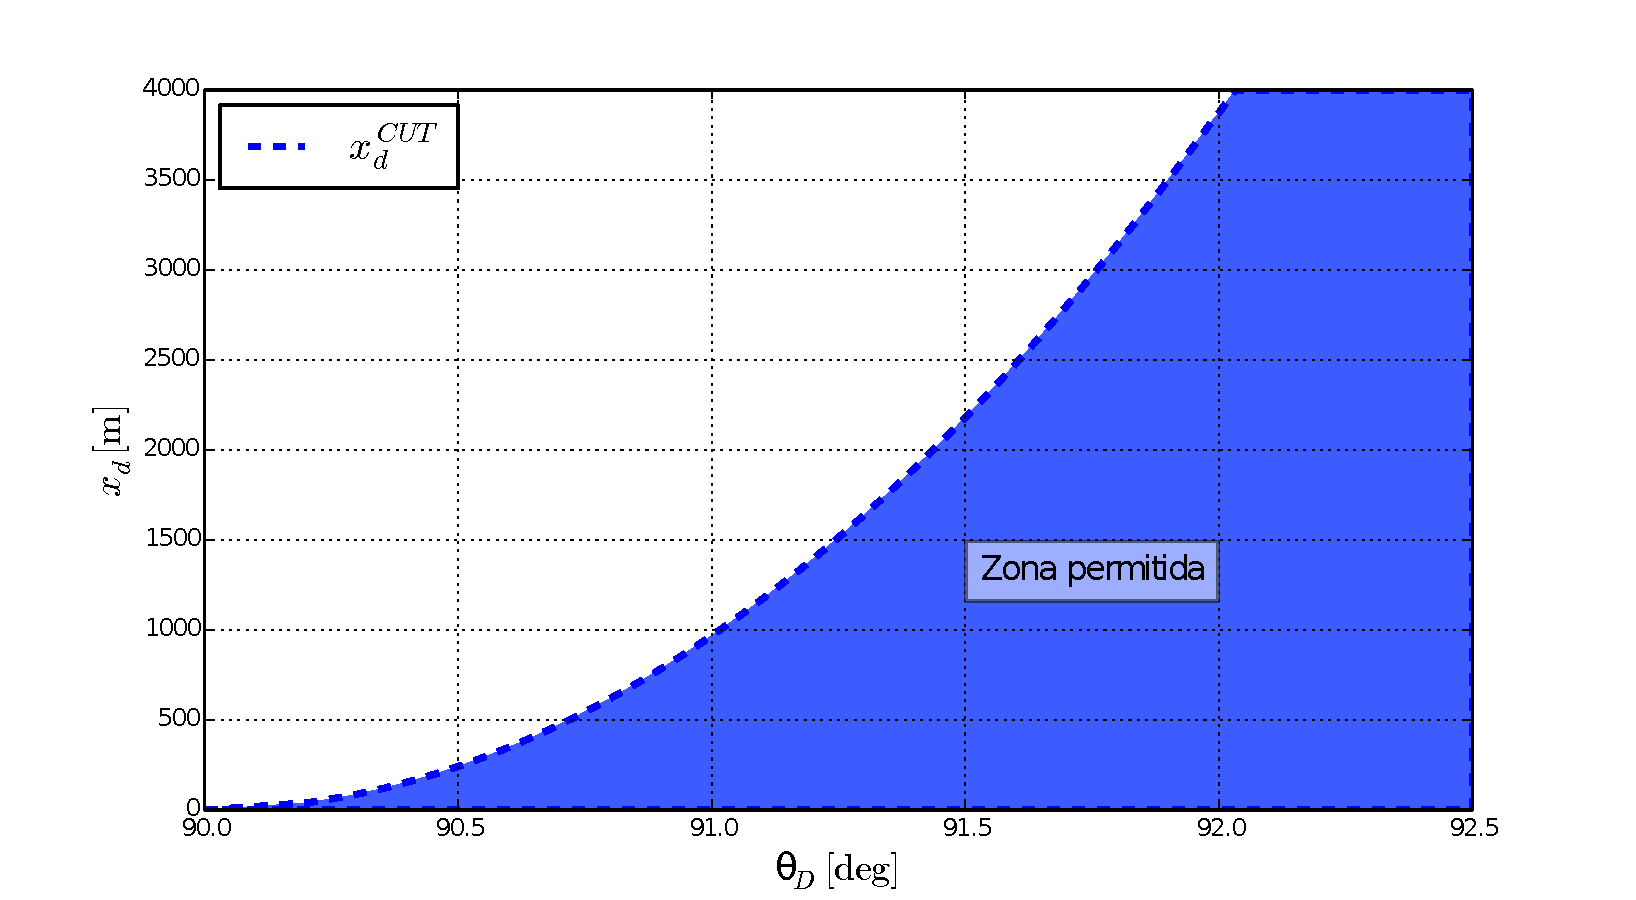
\includegraphics[width=0.95\textwidth]{./fig/appendix/thetaDCut_mod}
		% curveEarthSketch.png: 2404x1199 pixel, 150dpi, 40.70x20.30 cm, bb=0 0 1154 575
		\caption{\label{fig:dx_thcut0}
		Conjunto de par\'ametros geom\'etricamente admitidos.
		}
	\end{figure}
	%
	Si bien este efecto no tiene mucha relevancia en la exposici\'on de Auger\footnote{Esto se debe a que el rango angular en el que Auger es eficiente es de alrededor de $5^\circ$. Entonces, los eventos cuyo \'angulo se ve modificado siguen siendo detectados (ver figura \ref{fig:te_td} del apendice \ref{ap:tierraCurva}).}, tiene un impacto considerable en detectores de radio, cuyo rango angular de observaci\'on es cercano a los $2.5^\circ$.
	
	\subsection{Manejo de la energ\'ia visible}
	Las eficiencias de detecci\'on ser\'an calculadas en funci\'on de la energ\'ia visible de la lluvia, \ev{}, por lo que es necesario modificar el c\'alculo de la exposici\'on.
	Tomando como punto de partida las ecuaci\'ones \ref{eq:exp5ES} y \ref{eq:exp5.2ES} del cap\'itulo \ref{ch:resAuger}, el t\'ermino de probabilidad en este caso puede escribirse de la siguiente manera:
	%
	\begin{equation}
		\begin{aligned}
		P({\rm x_d},E_v|E_{\nu},\theta_D)=
		\int\limits_{E_v}^{E_\nu}
		g(E_v|E_\tau)
		& f(E_\tau|E_\nu,\theta_E(\theta_D,{\rm x_d}))\\
		&h({\rm x_d},(E_\tau,\theta_D))
		|\cos\theta_D|
		dE_\tau
		\end{aligned}
	\end{equation}
	%
	donde la funci\'on $f(E_\tau|E_\nu,\theta_E(\theta_D,{\rm x_d}))$ nuevamente describe la probabilidad de obtener un \tauon{} emergente de energ\'ia \etau{}, dado que incidi\'o un neutrino sobre la tierra de par\'ametros $E_\nu$ y $\theta_E(\theta_D,{\rm x_d})$, y al igual que en Auger se calcularon mediante simulaciones de Monte Carlo.
	Por otro lado $h({\rm x_d},(E_\tau,\theta_D))$ representa la probabilidad de decaimienta del \tauon{} en la atm\'osfera, descripta en la ecuaci\'on \ref{eq:decayTayRadio}, y $g(E_v|E_\tau)$ la probabilidad de que en ese decaimiento la lluvia se inicie energ\'ia \ev{} dado que el \tauon{} ten\'ia energ\'ia \etau{}.
	En lugar de $g(E_v|E_\tau)$, para realizar la integral se calcul\'o $\tilde{g}(\log E_v-\log E_\tau)$ a partir de la librer\'ia de \tauola{} utilizada para simular los decaimientos del \tauon{} en Auger.
	Esta funci\'on se muestra entre $-3$ y $0$ en la figura \ref{fig:ev_etau}, en la que se observa que aproximadamente el $95\%$ de los casos obtienen una energ\'ia visible a lo sumo un orden de magnitud menor que la del \tauon{}.
	%
	 \begin{figure}[h!]
		\begin{center}
			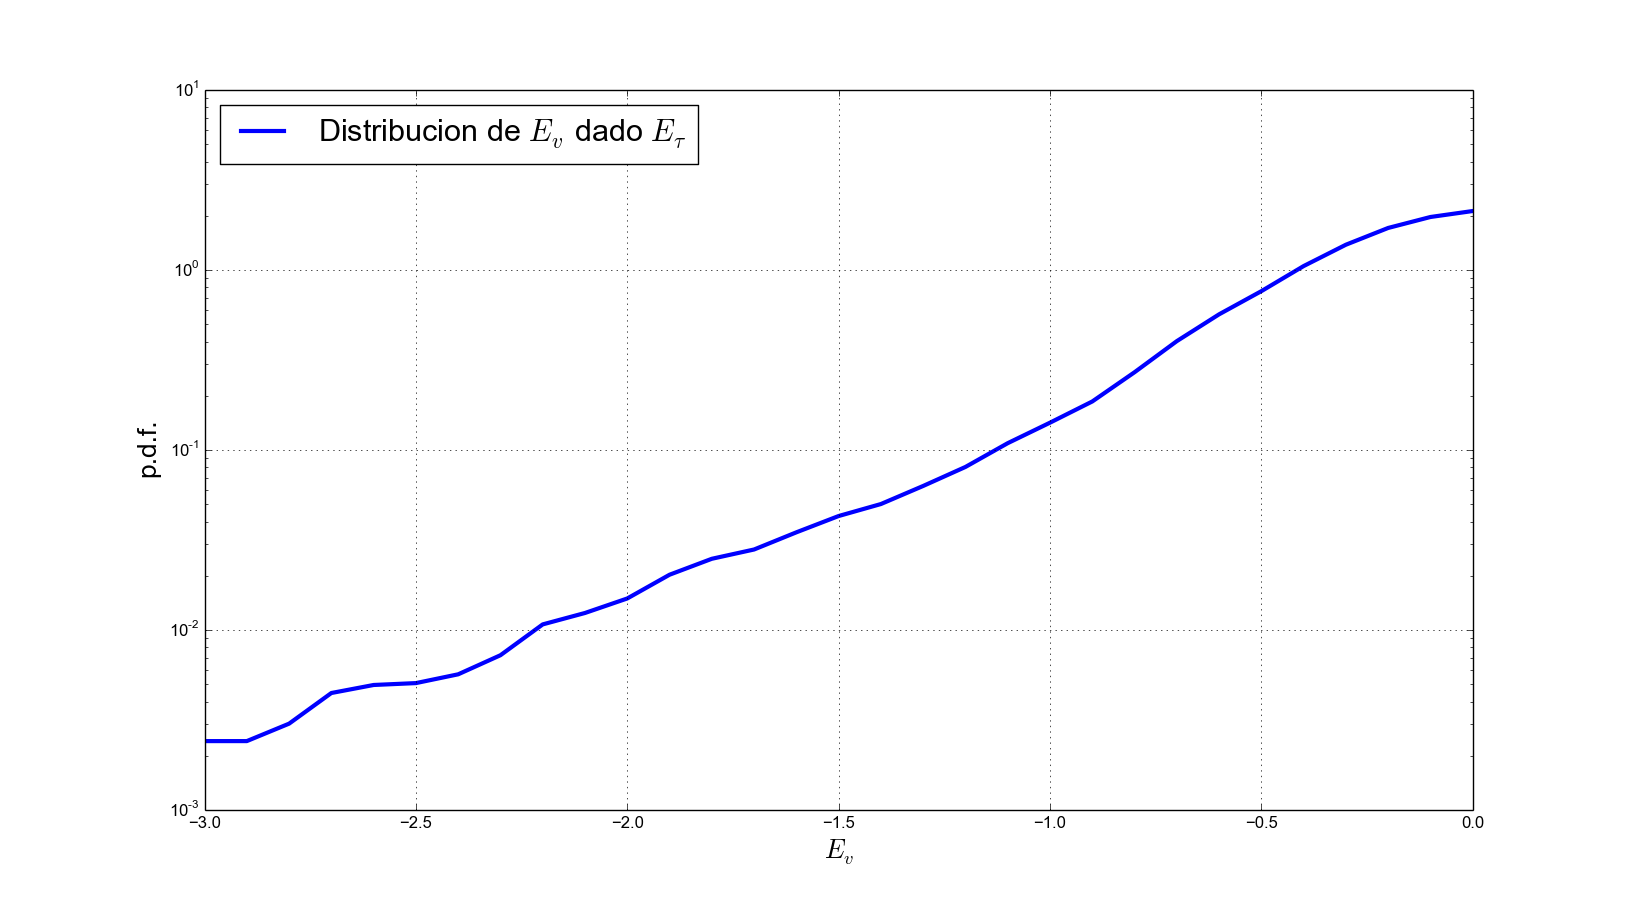
\includegraphics[width=0.9\textwidth]{fig/resultadosRadio/ev_etau}
			\caption{\label{fig:ev_etau} 
			Distribuci\'on de \ev{} dado \etau{} obtenida a partir de los decaimientos simulados con \tauola{}. 
			}
		\end{center}
	\end{figure}
	 
	\subsection{Integraci\'on temporal y espacial}
	Finalmente, dado que esta parte de la tesis se enfoca en un detector gen\'erico, no ser\'a necesario realizar la integral por unidad de tiempo y \'area y simplemente se multiplicar\'a por un factor \cant{T\ A=1}{s\,cm^2} o en caso de que se pretenda comparar con un detector, se utilizar\'a el factor correspondiente.
	
	Teniendo en cuenta todo lo anterior, la ecuaci\'on para calcular la exposici\'on resulta:
	%
	\begin{equation}
		\begin{aligned}
			{\cal E} (E_\nu) = 2 \pi T A
			\int_{0}^{\infty} 
			\int_{\theta_D^{cut}}^{\theta_D^{max}} 
			\int_{0}^{E_\nu} 
			\int_{0}^{E_\tau} 
			\epsilon ({\rm x_d},\theta_D,E_v)& 
			\frac{e^{\frac{l({\rm x_d})}{\lambda(E_\tau)}}}{\lambda(E_\tau)}\frac{dl({\rm x_d})}{d{\rm x_d}}
			\tilde{g}(\log E_v-\log E_\tau)\\
			f(E_\tau|E_\nu,\theta_E(\theta_D,{\rm x_d}))
			&\sin \theta_D |\cos \theta_D|
			dE_v dE_\tau  d\theta_D d{\rm x_d}
		\end{aligned}
		\label{eq:exp2ESRadio}
	\end{equation}

	Una vez obtenidas las eficiencias (ver secci\'on \ref{sc:effRadio}) esta integral se computa num\'ericamente.
	
	
\section{Detector ideal - corteza terrestre como blanco}
\label{sc:idealRadio}
	Antes de pasar al c\'alculo de las eficiencias de detecci\'on, es interesante estudiar las capacidades que tendria un detector ideal, es decir, que detecte todos los eventos iniciados por neutrinos ES que emerjan de la tierra.
	Para ello se calcul\'o la integral de la ecuaci\'on \ref{eq:exp2ESRadio} bajo la condici\'on $\epsilon ({\rm x_d},\theta_D,E_v) = 1$ y \cant{T\ A=1}{s\,cm^2}, para diferentes valores de $\theta_D^{max}$.
% 	Recordando la ecuaci\'on \ref{eq:exp0} del cap\'itulo \ref{ch:resAuger}, 
	En la figura \ref{fig:exposuresFluxThetas} se grafica esta cantidad multiplicada por $E_\nu^{-2}$, lo que, recordando la ecuaci\'on \ref{eq:exp0} del cap\'itulo \ref{ch:resAuger}, se debe integrar en $E_\nu$ para obtener la cantidad de eventos por unidad de \'area y tiempo~\footnote{Bajo la condici\'on de flujo unitario, es decir, $\Phi(E_{\nu})=k\,E_\nu^{-2}$ con \cant{k=1}{GeV\ s^{-1}\ sr^{-1}\ cm^{-2}}.}.
%
	\begin{figure}[h!]
		\begin{center}
			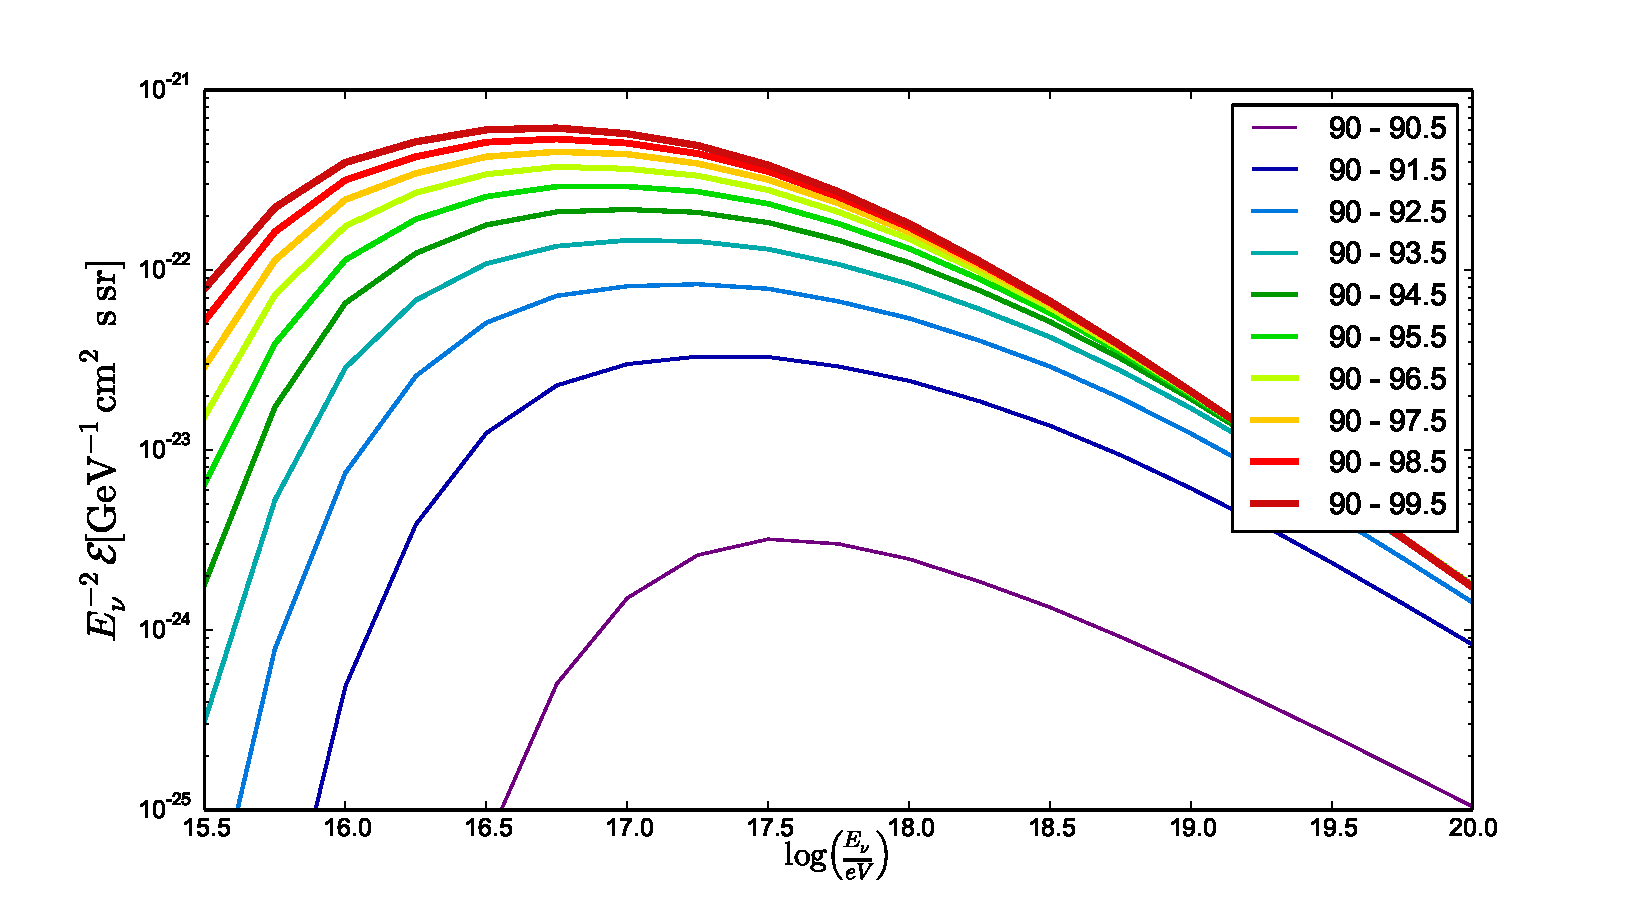
\includegraphics[width=0.9\textwidth]{fig/resultadosRadio/exposureFullEff_thetas}
			\caption{\label{fig:exposuresFluxThetas} Eventos esperados sobre el detector por unidad de \'area y tiempo para un flujo $\phi(E_\nu)= E^{-2}{\rm GeV\ s^{-1}\ sr^{-1}\ cm^{-2}}$, en funci\'on de la energ\'ia y suponiendo eficiencia m\'axima en el rango angular indicado.
			Naturalmente, la cantidad esperados aumenta a medida que lo hace el rango angular del \emph{detector ideal}.
			}
		\end{center}
	\end{figure}
	%
	
	Estas curvas representan la sensibilidad en energ\'ia del blanco, que como puede notarse, a medida que aumenta $\theta_D^{max}$ se desplaza hacia energ\'ias m\'as bajas.
	Este fen\'omeno se debe a que mientras mayor es el \'angulo de incidencia, los neutrinos m\'as energ\'eticos interactuar\'an en promedio m\'as lejos del lugar de escape hacia la atm\'osfera que los menos energ\'eticos\footnote{A medida que aumenta la energ\'ia del \nutau{} incidente la tierra se vuelve m\'as opaca.}, lo que le quita probabilidad de escapar al \tauon{} resultante.
	Por otro lado a medida que el rango angular de detecci\'on aumenta lo hace la cantidad de eventos esperados\footnote{El \'area bajo la curva aumenta con $\theta_D^{max}$.}.
	Para estudiar esta cantidad es posible realizar la integral en $E_\nu$ de cada curva, lo que se muestra en la figura \ref{fig:gainThetas} en unidades de la integral obtenida para el rango angular del detector de radio ($N_{92.5}$). 
	%
	\begin{figure}[h!]
		\begin{center}
			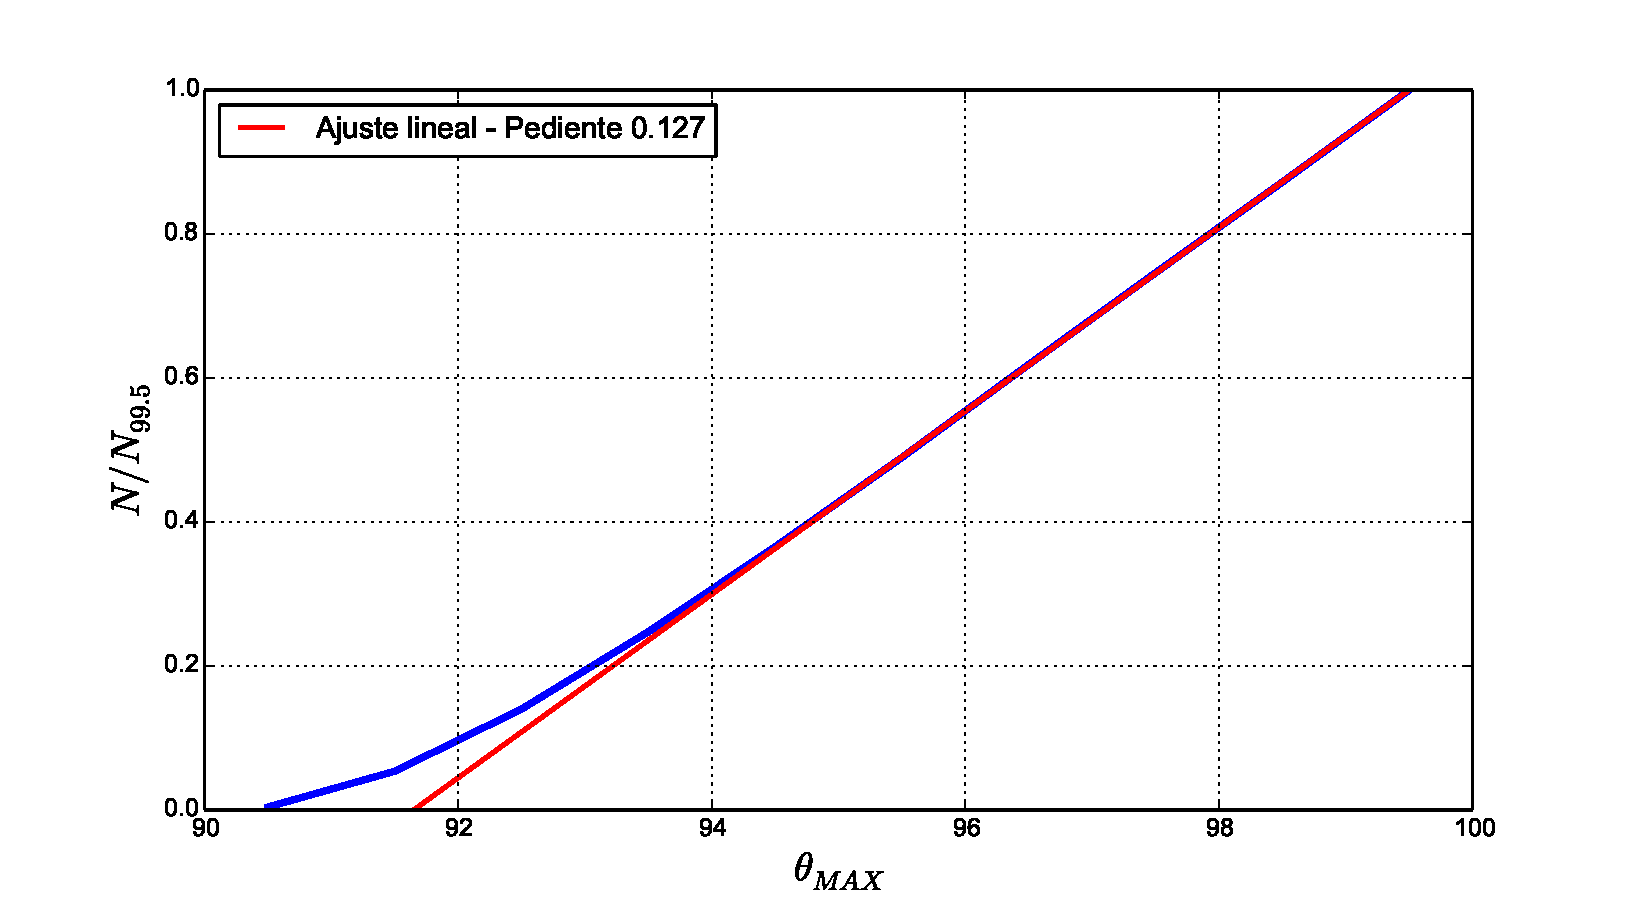
\includegraphics[width=0.9\textwidth]{fig/resultadosRadio/eventGain_thetas}
			\caption{\label{fig:gainThetas} Cantidad de eventos esperados como funci\'on del m\'aximo del rango angular, en relaci\'on al calculado para el del detector de radio ($N_{92.5}$).
			En rojo se grafica un ajuste lineal de pendiente 0.908, que aproxima la curva para valores de $\theta_{MAX}>94$.
			Esto quiere decir que cada grado por encima de $94^\circ$ aporta una cantidad constante eventos sobre el detector.
			}
		\end{center}
	\end{figure}
	%
	La primer observaci\'on interesante sobre la figura es que la relaci\'on entre $N(95^\circ)$ y $N(92.5^\circ)$ es aproximadamente 3.
	Esto quiere decir que en principio el detector de superficie de Auger tiene la capacidad de detectar el triple de eventos que uno equivalente basado en la t\'ecnica de radio.
	Esta desventaja debe ser compensada por un aumento significativo en el \'area instrumentada.
	
	Adem\'as, en la figura se muestra una recta de pendiente 0.908 obtenida mediante un ajuste lineal para los valores de $\theta_{MAX}>94$.
	Esto quiere decir que cada grado por encima de $94^\circ$ aporta una cantidad constante eventos sobre el detector (un $90\%$ de lo esperado para $\theta_D^{max}=92.5^\circ$).
	
\section{Obtenci\'on de las eficiencias}
\label{sc:effRadio}

Con el fin de calcular la integral de la ecuaci\'on \ref{eq:exp2ESRadio} es necesario obtener las eficiencias de detecci\'on a neutrinos en funci\'on de los par\'ametros $E_v$, $\theta_D$ y ${\rm x_d}$. 
Para ello, el enfoque elegido fue similar al desarrollado en el c\'alculo de Auger, que consisti\'o de los siguientes pasos:
%
\begin{enumerate}
	\item Simular la se\~nal a nivel del suelo para diferentes valores de $E_v$, $\theta_D$ y ${\rm x_d}$.
	\item \emph{Lanzar} la huella de radio sobre el detector varias veces en posiciones al azar.
	\item Calcular la fracci\'on de veces que la condici\'on de disparo global es alcanzada y as\'i obtener una eficiencia de disparo.
	\item Aplicar un criterio de selecci\'on a variables globales de cada evento y as\'i calcular una eficiencia de identificaci\'on.
\end{enumerate}
%

El cuello de botella en este c\'alculo result\'o ser el tiempo de CPU que requiere simular la se\~nal a nivel del suelo.
Esto es consecuencia de que para que la se\~nal se encuentre bien representada es necesario simular una superficie instrumentada de aproximadamente \cant{70\times3}{km} en la direcci\'on paralela y transversal a la direcci\'on de propagaci\'on de la lluvia respectivamente.
Asimismo, la granularidad no debe ser inferior a \cant{1000}{m} y \cant{100}{m} respectivamente, lo que implica que cada evento considerado necesita de la simulaci\'on de alrededor de 2000 antenas.
El tiempo que lleva realizar tal c\'alculo en las energ\'ias de inter\'es es cercano a los 10 dias de CPU por evento\footnote{Esta estimaci\'on corresponde a una CPU \texttt{Intel(R) Xeon(R) E5410 @ 2.33GHz}}, lo que puede volverlo r\'apidamente inviable si el n\'umero de lluvias a simular no es acotado.
En estas condiciones fue necesario utilizar todo el conocimiento obtenido hasta el momento para minimizar la cantidad de simulaciones realizadas.
El primer paso entonces fue estudiar la probabilidad relativa de ocurrencia de los eventos como funci\'on de $E_v$, $\theta_D$ y ${\rm x_d}$, lo que se desarrolla a continuaci\'on.
	
	\subsection{Pesos de las lluvias}
	Para determinar qu\'e bines (conjunto de valores $E_v$, $\theta_D$ y ${\rm x_d}$) es importante simular se calcul\'o la probabilidad relativa de ocurrencia, o lo que resulta equivalente, el peso relativo que tendr\'ia cada uno en la integral \ref{eq:exp2ESRadio} en un escenario de $\Phi(E_\nu)\propto E_\nu^{-2}$.
	Esta cantidad viene dada por:
	%
	\begin{equation}
		\begin{aligned}
			P_{sh}(E_v,\theta_D,{\rm x_d})
			\propto
			\sin{\theta_D}|\cos{\theta_D}|
			\iint\limits_{\mathbf{E_\tau}\mathbf{E_\nu}}&
			\frac{e^{\frac{l({\rm x_d})}{\lambda(E_\tau)}}}{\lambda(E_\tau)}\frac{dl({\rm x_d})}{d{\rm x_d}}
			%P({\rm x_d}|E_\tau;\theta_D)
			\tilde{g}(\log E_v-\log E_\tau)\\
			%P(\log{E_v}|\log{E_\tau})\\
			&f(E_\tau|E_\nu,\theta_E(\theta_D,{\rm x_d}))
			%&P(\log{E_\tau}|\log{E_\nu})
			E_\nu^{-2}
			dE_\tau dE_\nu
		\end{aligned}
		\label{eq:weightsRadio}
	\end{equation}
	%
	donde esta expresi\'on resulta de tener en cuenta todos los \nutau{}'s y \tauon{}'s que dan lugar a lluvias de par\'ametros $(E_v,\theta_D,{\rm x_d})$.
	Recordando el significado probabil\'istico de cada uno de los factores, se desprende que el valor de dicha integral es proporcional a la cantidad de eventos que se espera en las cercanias de cada punto del espacio de fases.
	%\footnote{Las integrales en $E_\nu$ y $E\tau$ dan cuenta de la suma sobre todos los neutrinos y taus que dan lugar a eventos de par\'ametros $(E_v^*,\theta_D^*,{\rm x_d}^*)$.}.
	Con esta medida es posible entonces establecer la importancia relativa entre diferentes bines.
	
	La figura \ref{fig:radioShWeights} muestra el resultado de la integral \ref{eq:weightsRadio} para diferentes valores de $E_v$, $\theta_D$ y ${\rm x_d}$.
	Se observa un decaimiento en la variable \xd{}, lo que es compatible con la probabilidad de decaimiento del \tauon{} en la atm\'osfera~\footnote{Esta se modela con una distribuci\'on exponencial.}. 
	Sin embargo a medida que aumenta la energ\'ia \'este se atenua, lo que es compatible con el hecho de que su longitud de decaimiento es proporcional a \etau{}.
	Por otro lado comprender el comportamiento en funci\'on de \td{} y \ev{} resulta complicado ya que mezcla la dependencia de las pdf (funci\'on $f(E_\tau|E_\nu,\theta_E(\theta_D,{\rm x_d}))$), el efecto de la tierra curva y la forma funcional del flujo de neutrninos, supuesto $\propto E^{-2}$.
	No obstante, este \'ultimo factor parece ser relevante ya que entre \cant{10^{16.25}}{eV} y \cant{10^{18.25}}{eV} los pesos caen cerca de dos \'ordenes de magnitud, lo que quiere decir que se
	Por este motivo no se utilizar\'an recursos para calcular con detalle las eficiencias por encima de \cant{10^{18}}{eV} y se las aproximar\'a por las obtenidas para esta energ\'ia, lo que constituye un enfoque conservador. 
	%
	\begin{figure}[ht!]
		\centering
		\begin{tabular}{cc}
		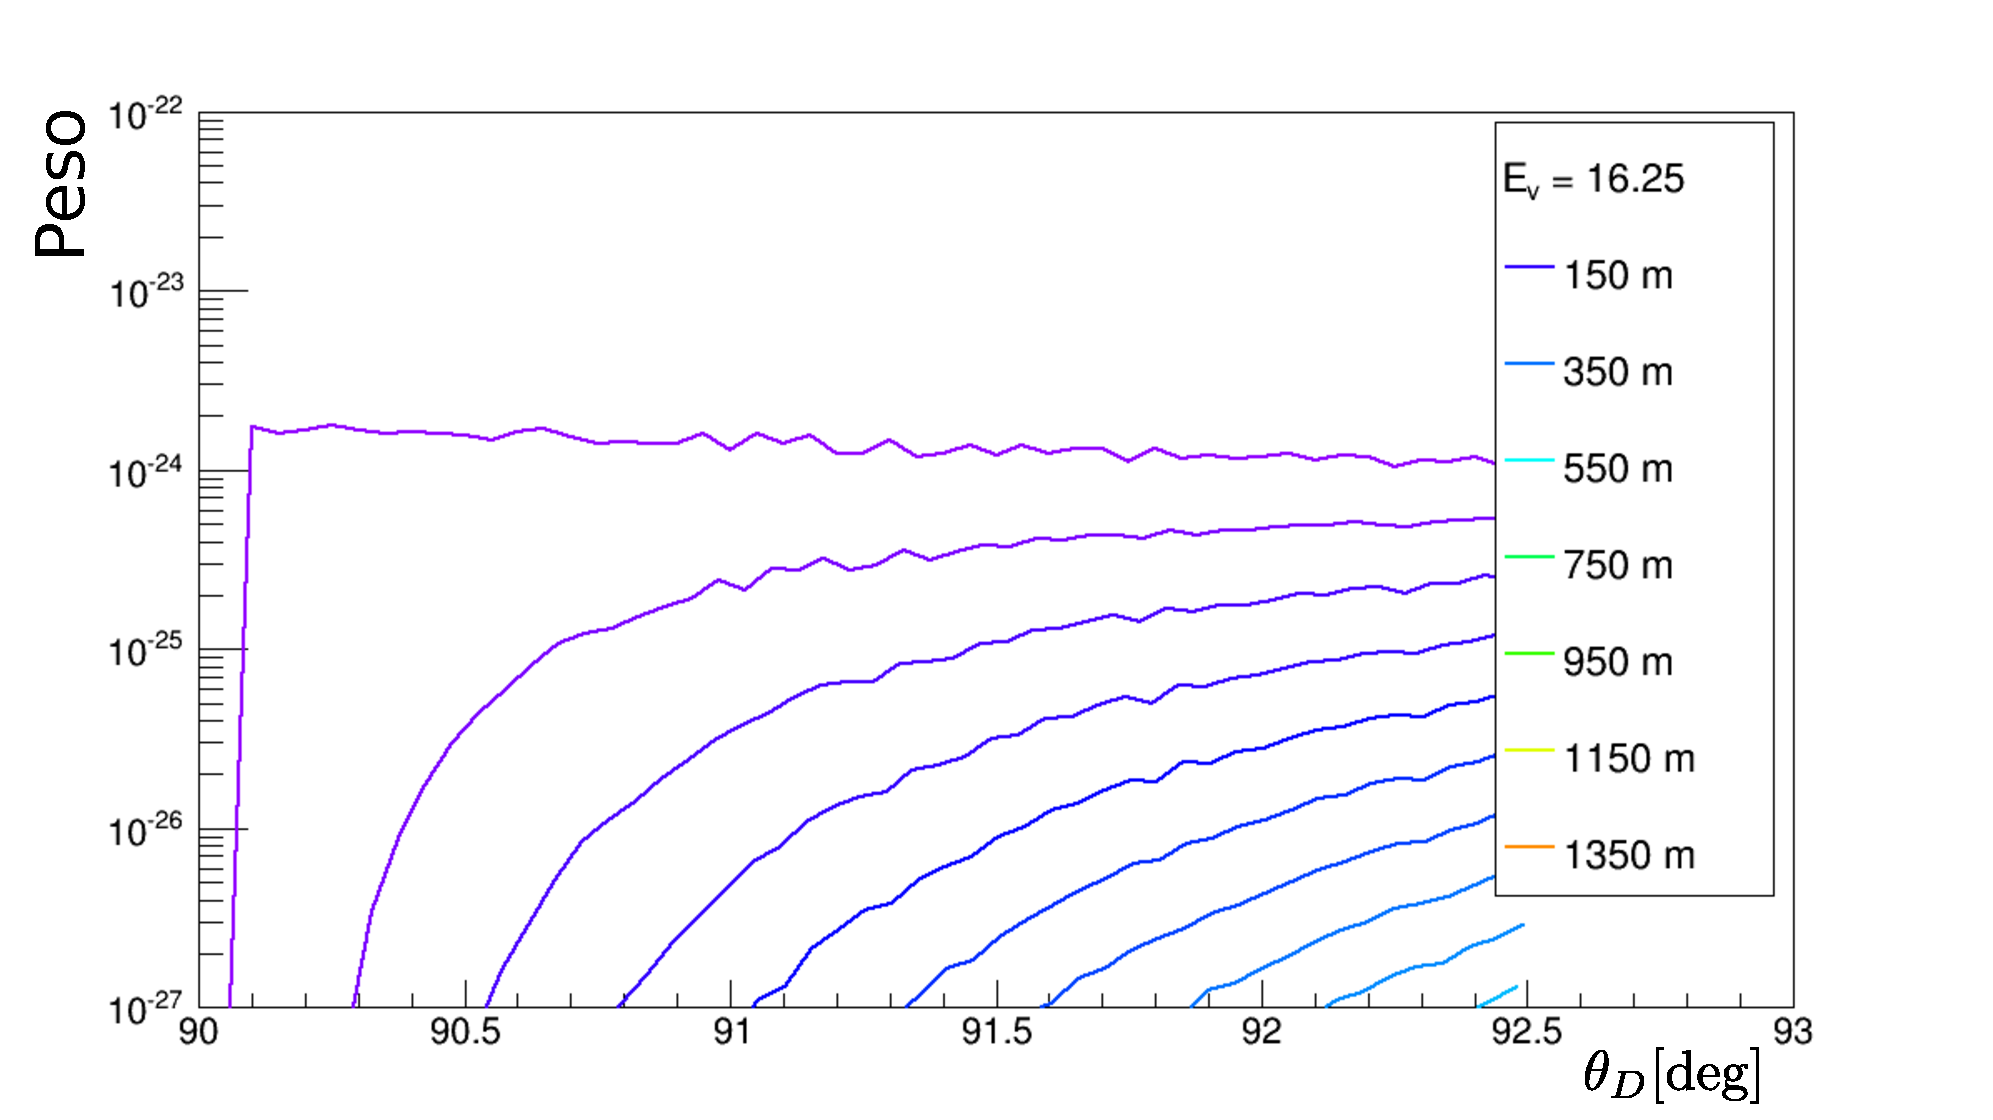
\includegraphics[width=0.45\textwidth]{fig/resultadosRadio/weights16_25} &
		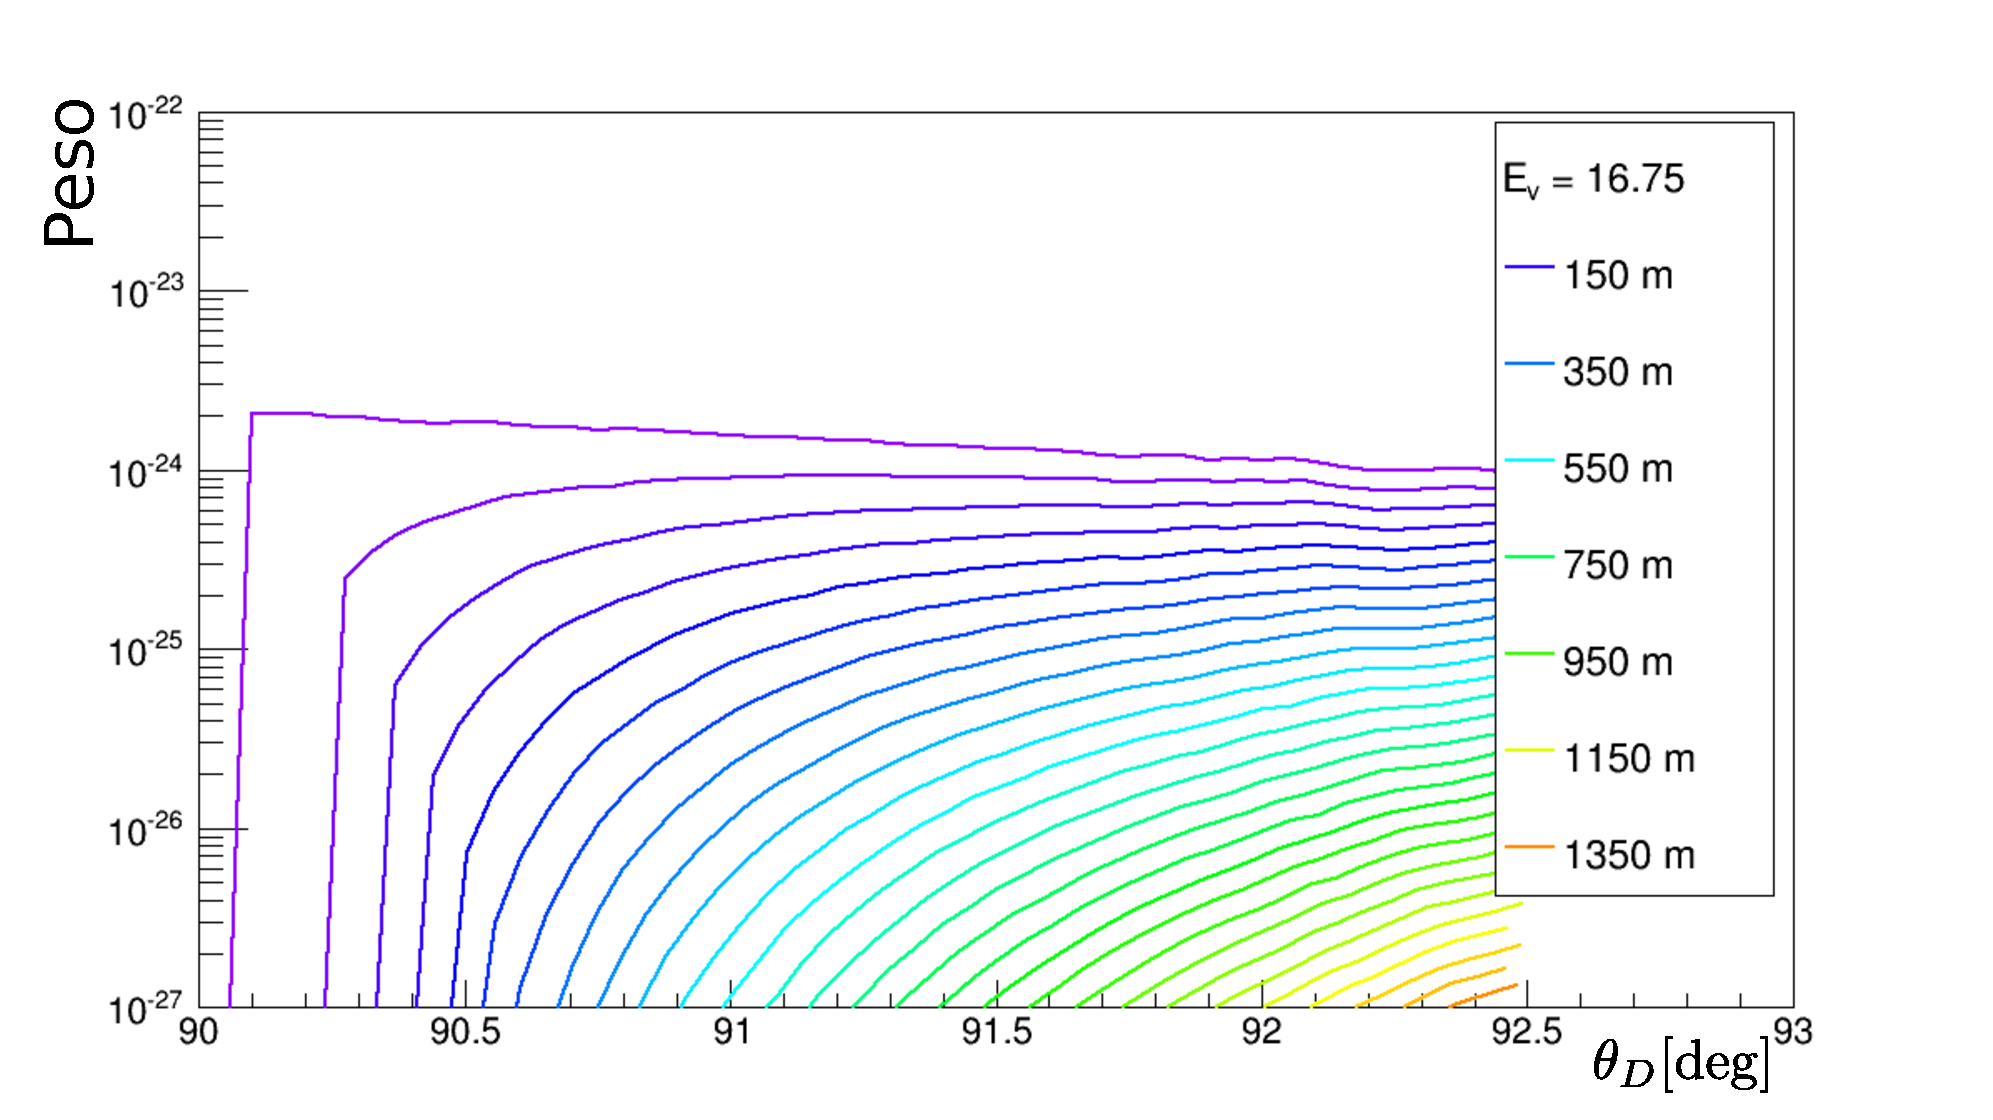
\includegraphics[width=0.45\textwidth]{fig/resultadosRadio/weights16_75} \\
		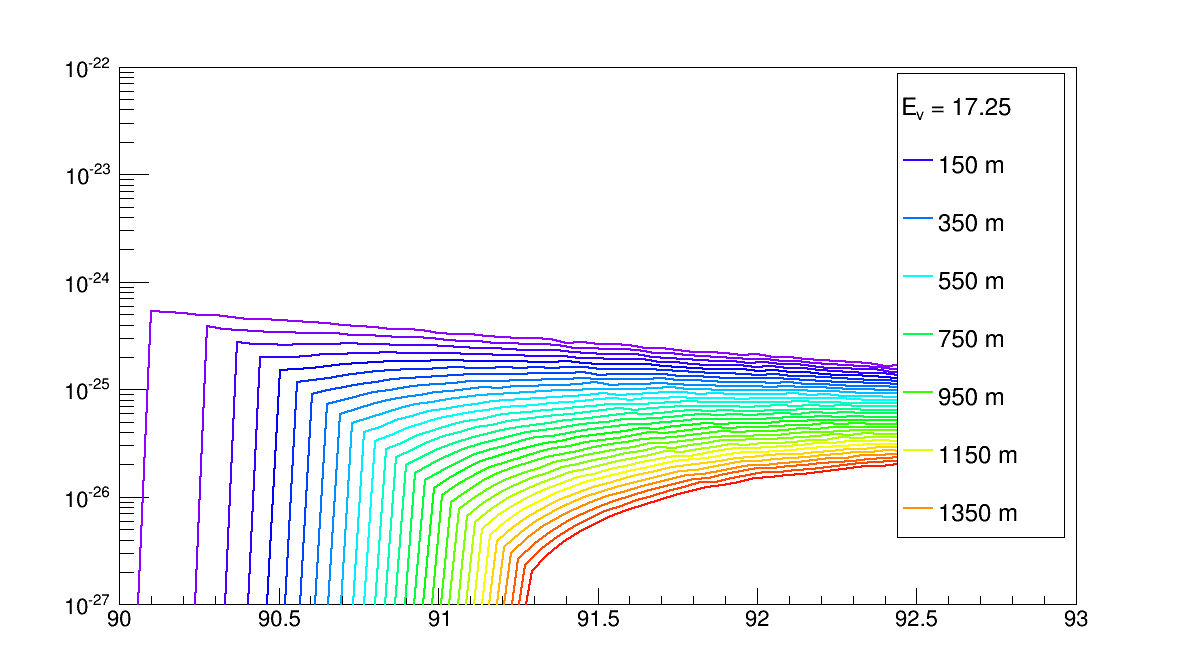
\includegraphics[width=0.45\textwidth]{fig/resultadosRadio/weights17_25} &
		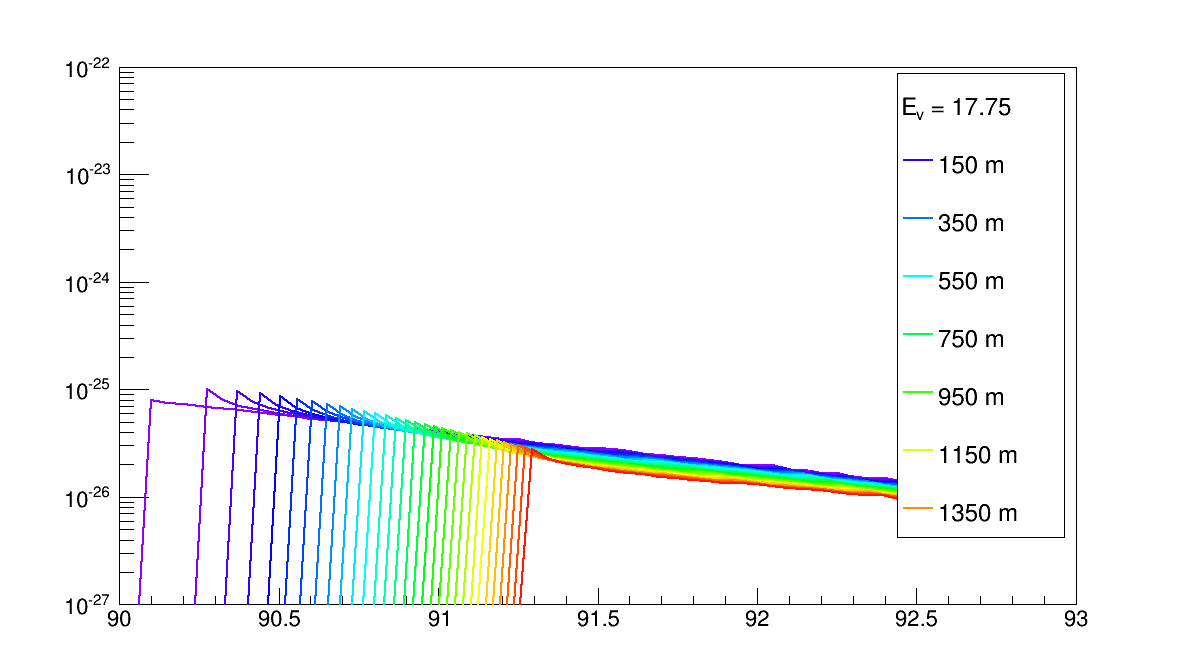
\includegraphics[width=0.45\textwidth]{fig/resultadosRadio/weights17_75} \\
		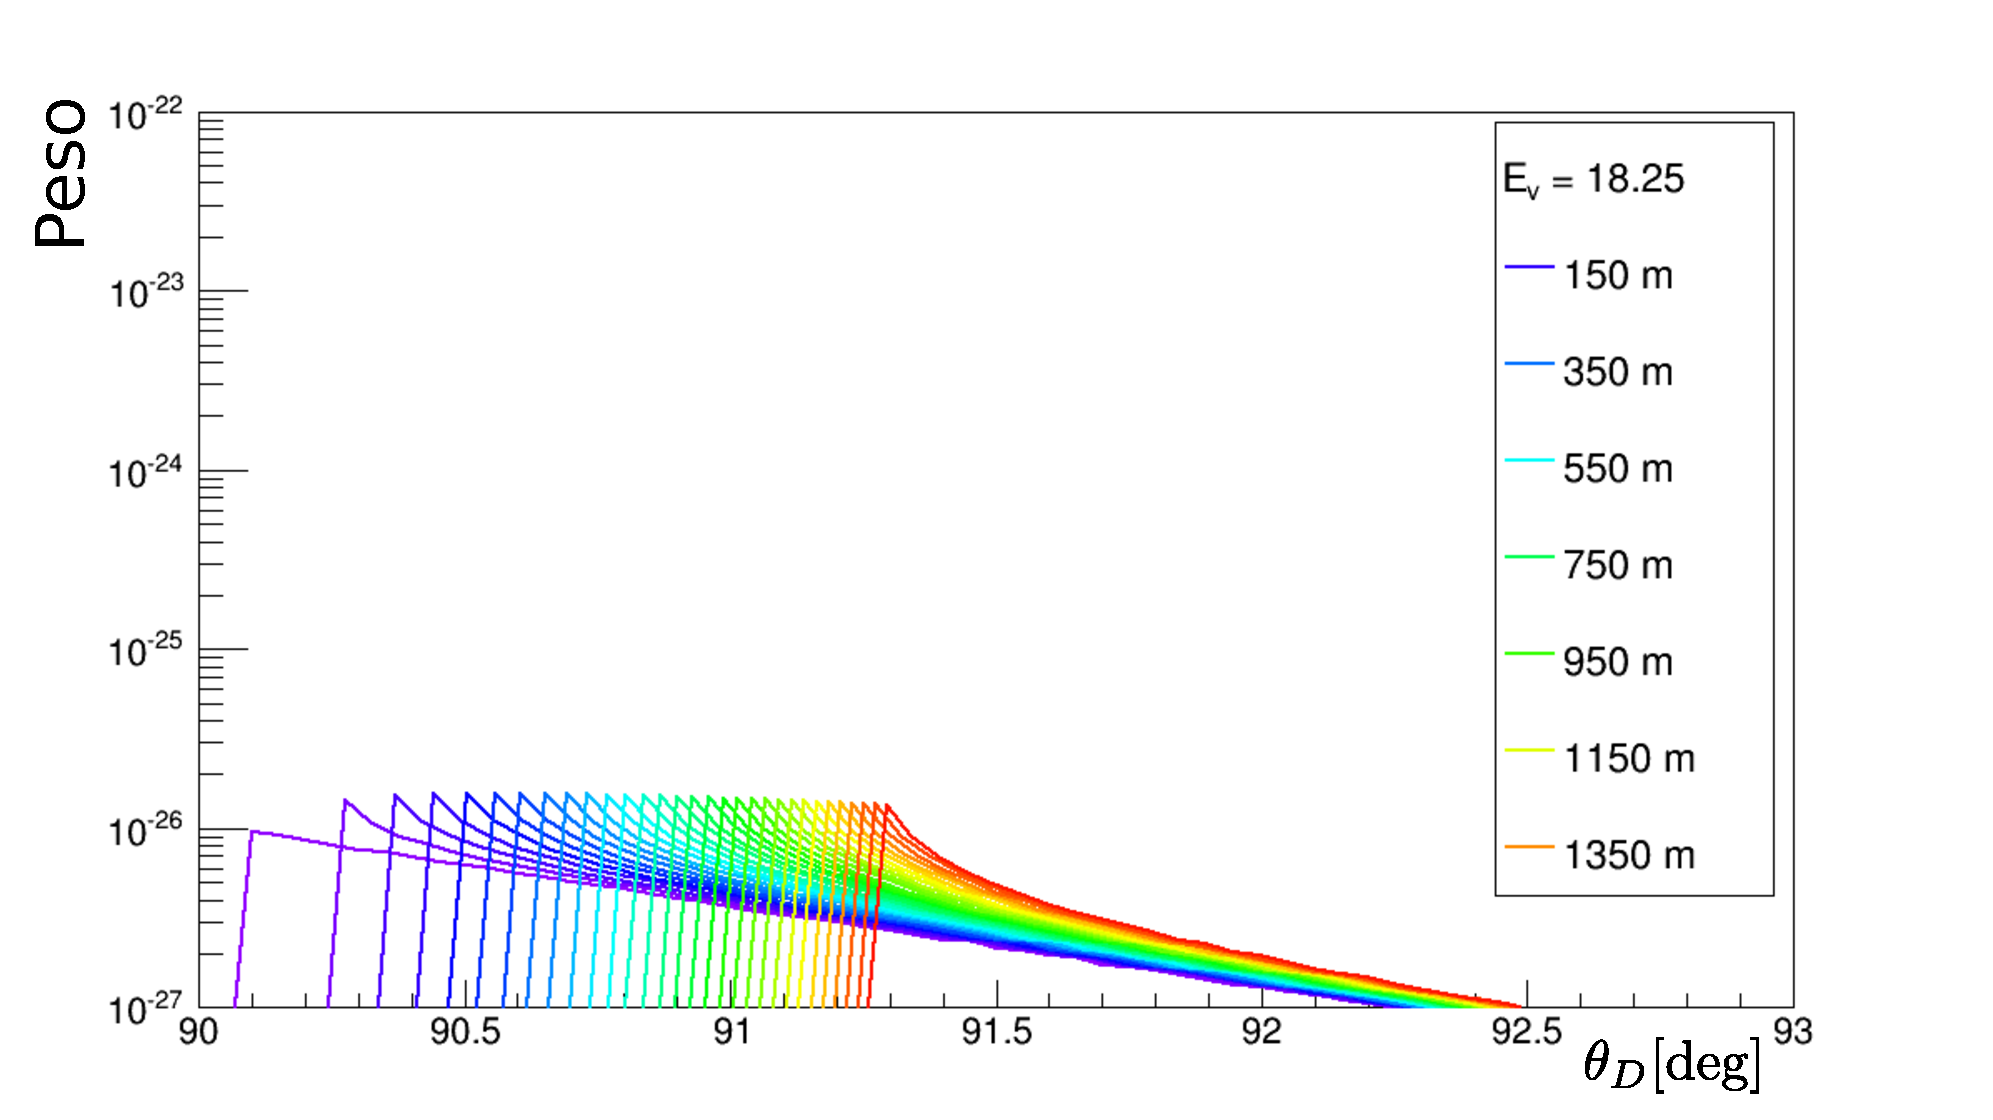
\includegraphics[width=0.45\textwidth]{fig/resultadosRadio/weights18_25} &
		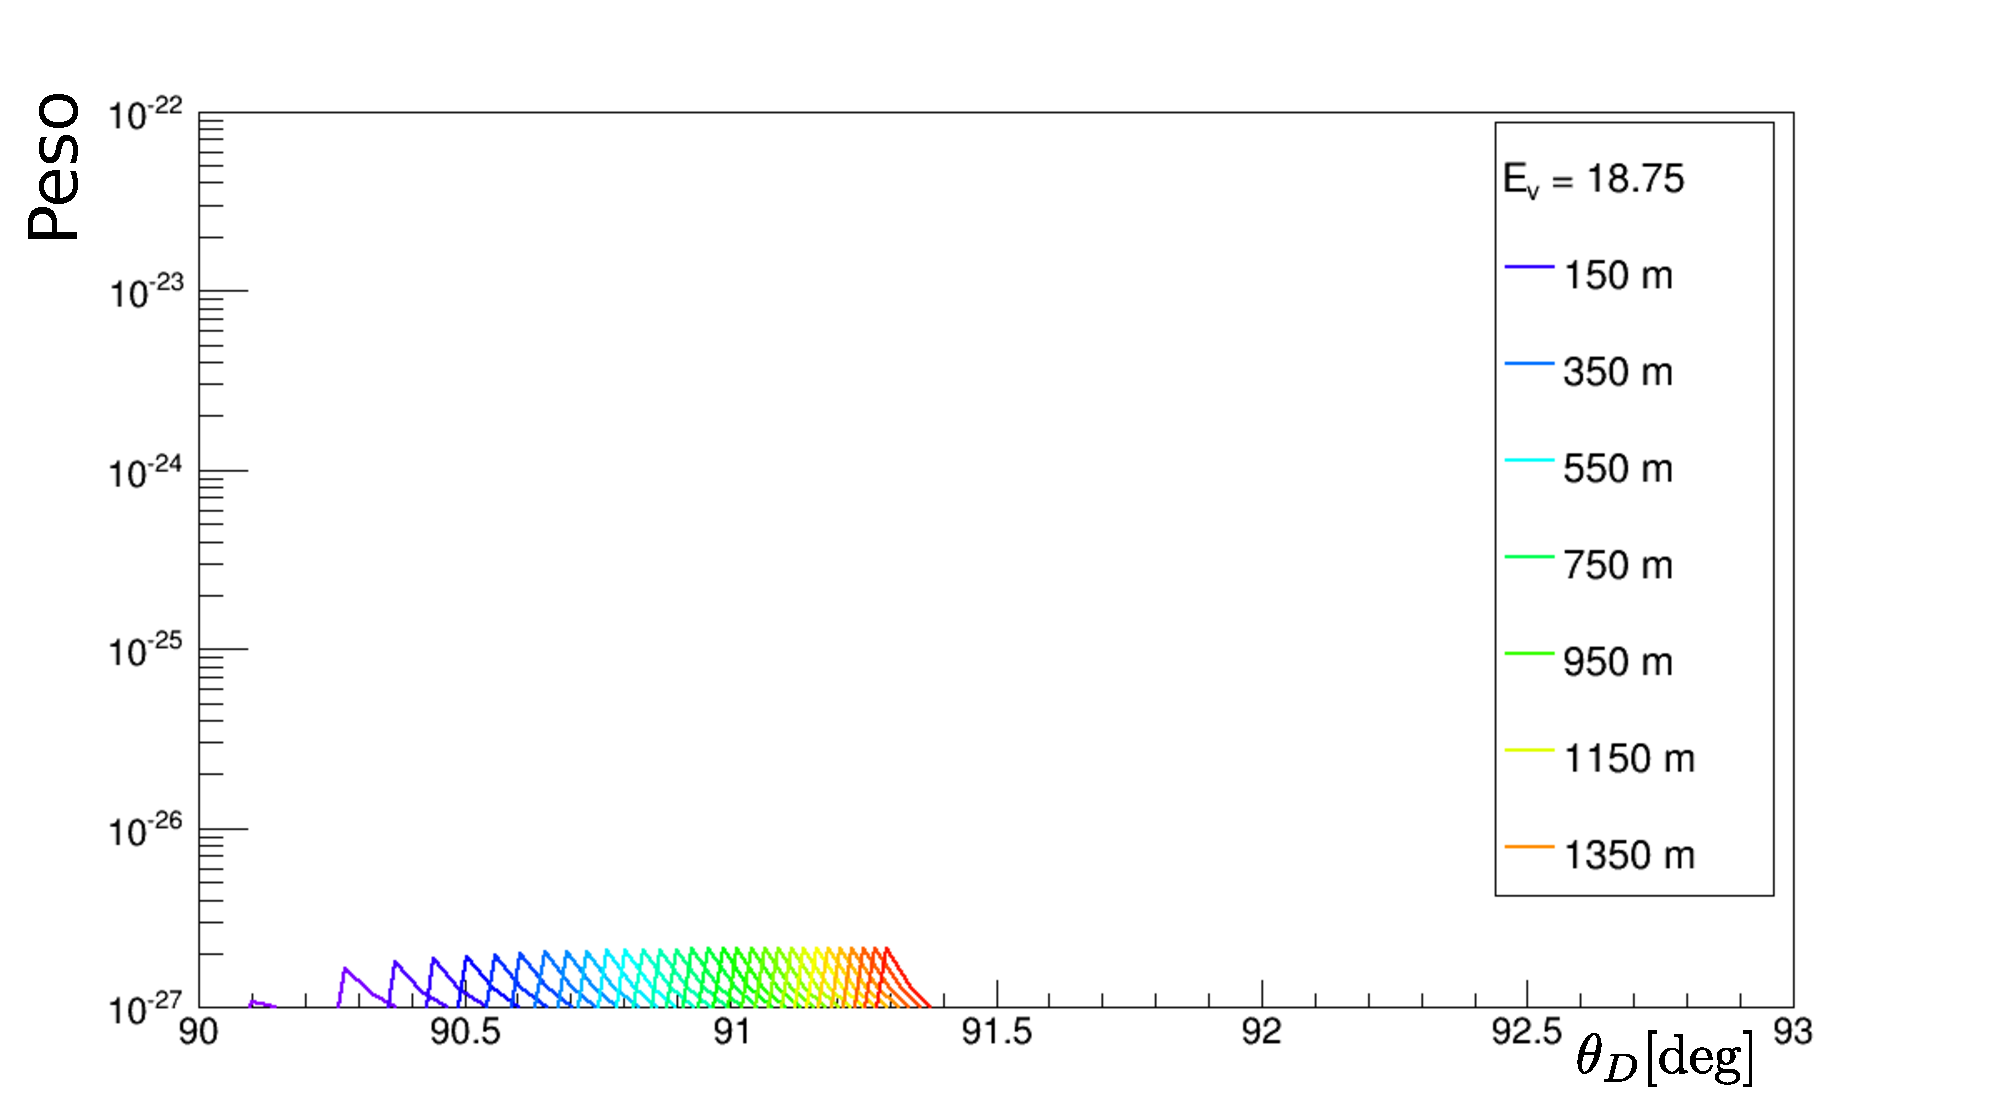
\includegraphics[width=0.45\textwidth]{fig/resultadosRadio/weights18_75} \\
		\end{tabular}

		\caption{\label{fig:radioShWeights}
		Probabilidad relativa  de las lluvias en funci\'on de la altura de decaimiento y el \'angulo cenital para diferentes valores de energ\'ia visible, suponiendo un flujo $\Phi(E_\nu)\propto E^{-2}$ y eficiencia m\'axima.
		Estos gr\'aficos muestran la importancia relativa en la exposici\'on de los diferentes bines de energ\'ia visibles, \'angulos cenitales y alturas de decaimiento.
		Por ejemplo, para $\sim90^\circ$ y \cant{150}{m} se esperan del orden de 100 veces m\'as eventos a \cant{10^{17.25}}{eV} que a \cant{10^{18.25}}{eV}.
		}
	\end{figure}
	
	\subsection{Espacio de par\'ametros simulado}
	
	En base a lo expuesto hasta el momento y en el cap\'itulo \ref{ch:caracterizacionRadio}, se tuvieron en cuenta las siguientes consideraciones para determinar el espacio de par\'ametros sobre el que calcular las eficiencias de disparo:
	%
	\begin{enumerate}
		\item La simulaci\'on de cada evento ES sobre un detector que permita representar de manera fidedigna la huella a nivel del suelo es extremadamente costosa computacionalmente, de alrededor de 230 horas de CPU por evento.
		Por esta raz\'on se intent\'o minimizar la cantidad de eventos simulados.
		\item El \'angulo sobre el detector se simular\'a entre el \'angulo m\'inimo admitido para cada valor de \xd{} (seg\'un figura \ref{fig:dx_thcut0}) y $92.5^\circ$, de acuerdo con lo discutido en la secci\'on \ref{sbsc:depThetaRadio}.
		\item Si bien la probabilidad de disparo de la lluvia aumenta a medida que lo hace la energ\'ia visible (ver secci\'on \ref{sbsc:depEvRadio}), de acuerdo con la figura \ref{fig:radioShWeights} la importancia de un evento de \cant{E_v=10^{18}}{eV} resulta ser aproximadamente dos \'ordenes de magnitud menor que uno tal que \cant{E_v=10^{16}}{eV}. Por este motivo no se simular\'an eventos cuya energ\'ia visible supere los \cant{10^{18}}{eV}. 
		\item Para determinar las alturas de decaimiento a simular se analiz\'o para cada valor de \ev{} el campo el\'ectrico m\'aximo de la huella (de acuerdo con lo expuesto en la secci\'on \ref{sbsc:depXdRadio}) en combinaci\'on con la probabilidad de ocurrencia de la figura \ref{fig:radioShWeights}. Se evit\'o la simulaci\'on de eventos poco probables o sin posibilidad de disparar antenas.
	\end{enumerate}
	
	En Auger, la eficiencia en el \'angulo azimutal $\phi$ y en el canal de decaimiento del \tauon{} se obtuvo en promedio al simular varias lluvias para cada bin de $\theta$, \xd{} y \etau{}.
	Dado que aqu\'i se requiere minimizar la cantidad de eventos simulados, se utiliz\'o para todos $\phi=0^\circ$ como \'angulo azimutal y $\tau\rightarrow\nu_\tau e^-\nu_e$ canal de decaimiento del \tauon{}.
	La primer elecci\'on resulta conservadora seg\'un lo expuesto en la secci\'on \ref{sbsc:depPhiRadio}, mientras que la segunda parece ser una buena estimaci\'on del promedio en esa variable seg\'un la secci\'on \ref{sbsc:decayChRadio}.
	
	Tendiendo todo esto en cuenta se simul\'o un evento para cada bin de $E_v$, $\theta_D$ y ${\rm x_d}$ que se grafica en la figura \ref{fig:binesRadio}.
	En total la simulaci\'on requiri\'o alrededor de 7500 dias de CPU, lo que tom\'o alrededor de un mes de calendario en el cluster de la Universidad de Santiago de Compostela, que cuenta con 500 nodos compartidos entre varios grupos de investigaci\'on. 
	%
	\begin{figure}[h!]
		\begin{center}
			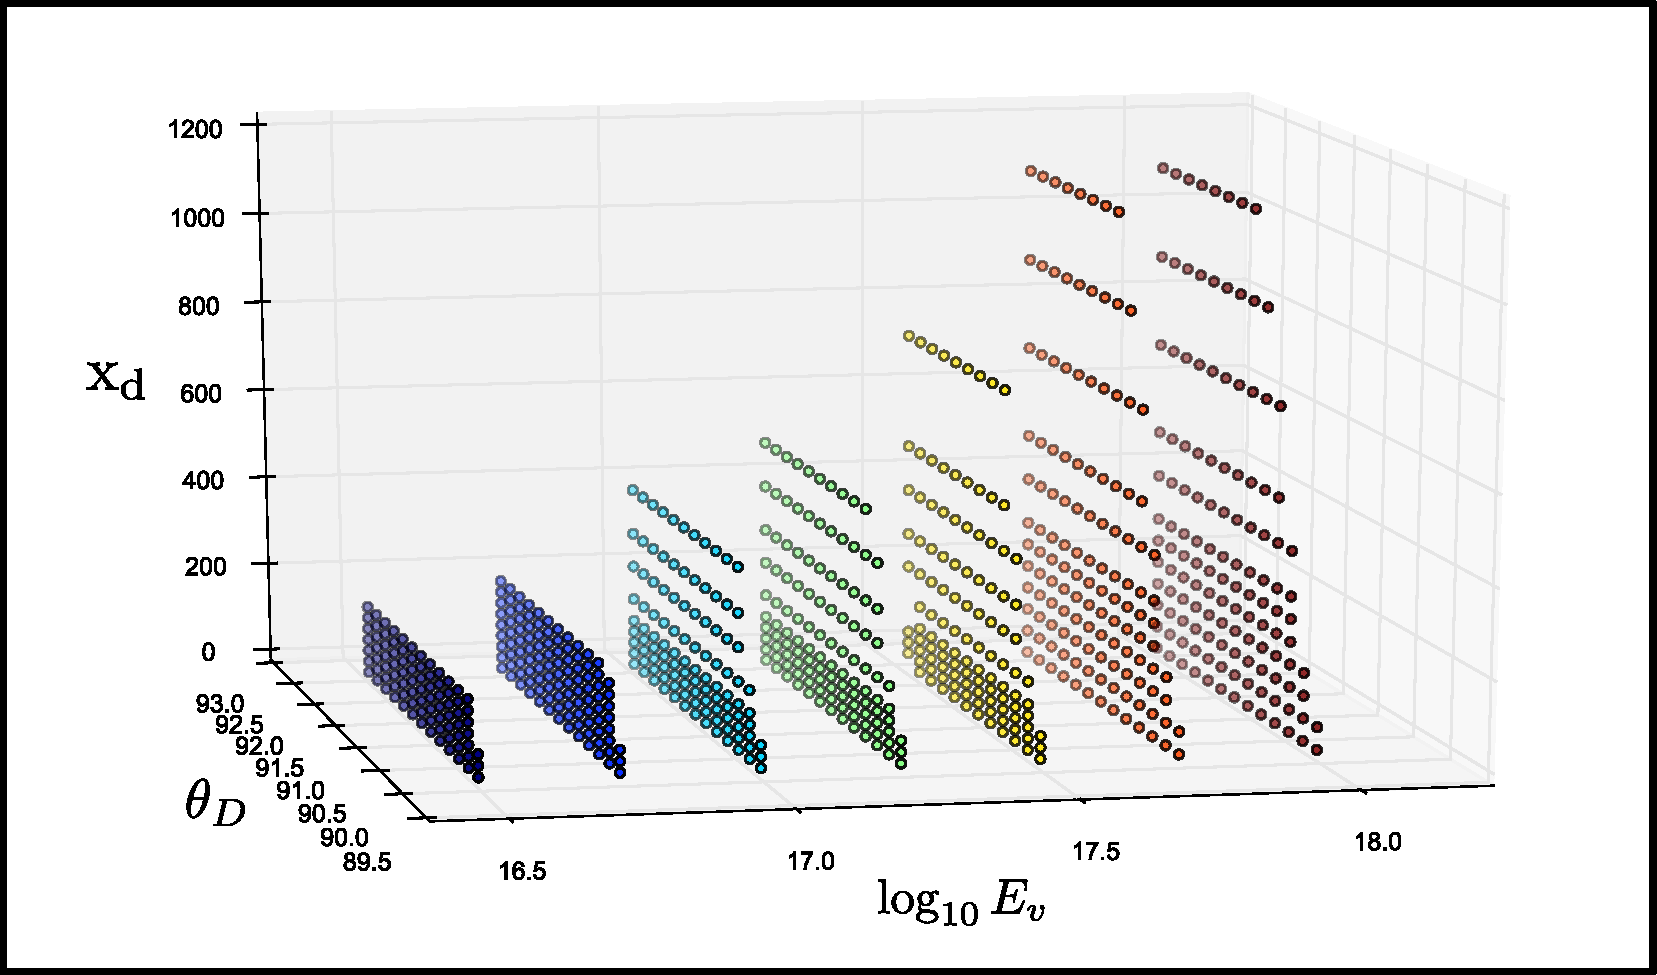
\includegraphics[width=0.9\textwidth]{fig/resultadosRadio/binesRadio_3}
			\caption{\label{fig:binesRadio} Espacio de par\'ametros cubierto donde se calcularon las eficiencias de disparo. Cada punto indica una lluvia simulada.
			}
		\end{center}
	\end{figure}
	
	\subsection{Topograf\'ia del detector}
	
	Una vez obtenida la se\~nal a nivel del suelo para todo el espacio de par\'ametros, el siguiente paso es definir la topograf\'ia del detector, es decir, la distribuci\'on de antenas en la superficie.
	Para ello se consideraron tres familias distintas, que se bosquejan en la figura \ref{fig:topoRadio} y se describen a continuaci\'on:
	%
	\begin{description}
	 \item[Regular:] Consiste en un arreglo bidimensional definido por dos pasos $a_1$ y $a_2$, y un \'angulo $\alpha$. Por ejemplo el SD de Auger es un arreglo de este tipo con \cant{a_1=a_2=1500}{m} y $\alpha=60^\circ$.
	 \item[Tipo panal de abeja:] Igual que el anterior pero con un detector faltante cada tres, por lo que permite cubrir una mayor superficie con la misma cantidad de antenas a costa de una p\'erdida de eficiencia debido a la baja en la granularidad. Nuevamente se parametriza con los pasos $a_1$ y $a_2$, y el \'angulo $\alpha$. 
	 \item[Bordes densos:] Este tipo de arreglo busca sacar ventaja de las dos dimensiones presentes en la huella de radio. Dependiendo de los valores que tomen los par\'ametros $D$ y $d$ la superficie cubierta puede ser mayor o menor que un arreglo regular para la misma cantidad de celdas de detecci\'on.  
	\end{description}
	%
	\begin{figure}[h!]
		\begin{center}
			\includegraphics[width=0.75\textwidth]{fig/resultadosRadio/topografia}
			\caption{\label{fig:topoRadio} Topograf\'ias estudiadas al calcular las eficiencias. Tanto el arreglo regular como el tipo panal de abeja se parametrizan mediante los pasos $a_1$ y $a_2$, y el \'angulo $\alpha$. Por otro lado, el arreglo de bordes densos queda determinado por los pasos mayor y menor $D$ y $d$.
			}
		\end{center}
	\end{figure}
	
% 	\begin{figure}[h!]
% 		\begin{center}
% 		\begin{tabular}{cc}
% 			\cant{a_1=a_2=1000}{m}, $\alpha=90^\circ$ &
% 			\cant{a_1=a_2=1500}{m}, $\alpha=60^\circ$ \\
% 			\includegraphics[width=0.5\textwidth]{fig/resultadosRadio/{17.00_89.90_00.00_00025_01238_1000_1000_90_re}.pdf} &
% 			\includegraphics[width=0.5\textwidth]{fig/resultadosRadio/{17.00_89.90_00.00_00025_01238_1500_1500_60_re}.pdf} \\
% 			\cant{a_1=a_2=750}{m}, $\alpha=60^\circ$ &
% 			\cant{d=250}{m}, \cant{D=4000}{m} $\alpha=60^\circ$ \\
% 			\includegraphics[width=0.5\textwidth]{fig/resultadosRadio/{17.00_89.90_00.00_00025_01238_750_750_60_hc}.pdf} &
% 			\includegraphics[width=0.5\textwidth]{fig/resultadosRadio/{17.00_89.90_00.00_00025_01238_250_4000_90_de}.pdf}
% 		\end{tabular}
% 			\caption{asd}
% 			\label{fig:}
% 		\end{center}
% 	\end{figure}
	
	
	\subsection{Eficiencias de disparo}
	
	Las eficiencias de disparo se calcularon mediante un m\'etodo similar al empleado en Auger.
	Se lanz\'o cada una de las se\~nales simuladas sobre un detector \emph{infinito} cuya topograf\'ia fue definida como en la secci\'on anterior.
	El procedimiento se describe a continuaci\'on:
	\begin{enumerate}
	 \item Dada la topograf\'ia del detector se defini\'o una celda primitiva, es decir, un conjunto de antenas y una regi\'on del suelo que represente una unidad de detecci\'on m\'inima.
	 \item Para cada lluvia se calcul\'o el baricentro de la se\~nal y se lo lanz\'o 1000 veces en posiciones al azar dentro de dicha celda.
	 \item Se rot\'o la se\~nal en un \'angulo $\phi$ se eligido al azar~\footnote{Si bien la se\~nal fue simulada utilizando $\phi=0^\circ$, es necesario sortear el \'angulo azimutal para incluir en el c\'alculo la anisotrop\'ia del detector.}.
	 \item Para determinar qu\'e antenas del detector fueron disparadas se asign\'o a cada una la se\~nal del observador simulado m\'as cercano, siempre y cuando este se encontrase a menos de \cant{500}{m} en direcci\'on forward y \cant{50}{m} en direcci\'on transversal.
% 	 \item Se corrigi\'o el tiempo del m\'aximo de la se\~nal, que luego ser\'a el tiempo de disparo, seg\'un la distancia en la direcci\'on forward, en unidades de la velocidad de la luz.
	 \item Para evaluar la condici\'on de disparo local se utiliz\'o un valor fijo, de acuerdo con lo discutido en la secci\'on \ref{sbsc:localTriggerRadio}, que vari\'o entre \cant{25}{\frac{\mu V}{m}} y \cant{250}{\frac{\mu V}{m}}.
	 \item Finalmente como condici\'on de disparo global se requiri\'o una m\'inima cantidad de antenas disparadas. Se repiti\'o el procedimiento pidiendo al menos 3, 5, 7 y 9 antenas disparadas.
	\end{enumerate}

	En las figuras \ref{fig:corePos1} y \ref{fig:corePos2} se muestran las posiciones de generadas para una de las lluvias en distintas topograf\'ias.
	En la figura \ref{fig:corePos1} se grafican sobre un arreglo regular cuadrado, con \cant{a_1=a_2=1000}{m} y $\alpha=90^\circ$, y uno regular como el del SD de Auger, es decir, \cant{a_1=a_2=1500}{m}y $\alpha=60^\circ$.
	Por otra parte, en la figura \ref{fig:corePos2} se muestran para un arreglo tipo panal de abeja \cant{a_1=a_2=750}{m} y $\alpha=60^\circ$, y para uno de bordes densos con \cant{d=500}{m}, \cant{D=4000}{m}.
	%
	\begin{figure}[ht!]
		\begin{center}
		\begin{tabular}{cc}
			\cant{a_1=a_2=1000}{m}, $\alpha=90^\circ$ \\
			\includegraphics[width=0.8\textwidth]{fig/resultadosRadio/{17.00_89.90_00.00_00025_01238_1000_1000_90_re}.pdf} \\
			\cant{a_1=a_2=1500}{m}, $\alpha=60^\circ$ \\
			\includegraphics[width=0.8\textwidth]{fig/resultadosRadio/{17.00_89.90_00.00_00025_01238_1500_1500_60_re}.pdf} \\
		\end{tabular}
			\caption{\label{fig:corePos1}
			Arriba, una grilla cuadrada de \cant{1000}{m} de paso. Abajo, una grilla hexagonal centrada de \cant{1500}{m} de paso como la del SD de Auger.
			En rojo se muestra la posici\'on del baricentro de la lluvia, lanzado al azar de 1000 dentro de la correspondiente celda primitva.
			}
		\end{center}
	\end{figure}
	%
	\begin{figure}[ht!]
		\begin{center}
		\begin{tabular}{cc}
			\cant{a_1=a_2=750}{m}, $\alpha=60^\circ$ \\
			\includegraphics[width=0.8\textwidth]{fig/resultadosRadio/{17.00_89.90_00.00_00025_01238_750_750_60_hc}.pdf} \\
			\cant{d=500}{m}, \cant{D=4000}{m}\\
			\includegraphics[width=0.8\textwidth]{fig/resultadosRadio/{17.00_89.90_00.00_00025_01238_500_4000_90_de}.pdf}
		\end{tabular}
			\caption{\label{fig:corePos2}
			Arriba, una grilla hexagonal tipo panal de abeja de \cant{750}{m} de paso. Abajo, una de tipo bordes densos de \cant{4000}{m} de paso y \cant{500}{m} de paso interno.
			Nuevamente en rojo se muestra la posici\'on del baricentro de la lluvia, lanzado al azar de 1000 dentro de la correspondiente celda primitva.}
		\end{center}
	\end{figure}
	
	En la figura \ref{fig:globalTriggerRadio} se muestra el resultado de un lanzamiento de una lluvia de \cant{E_v=10^{18}}{eV}, $\theta_D=90.5^\circ$ y \cant{{\rm x_d}=25}{m} sobre un arreglo regular de \cant{a_1=a_2=1000}{m} y $\alpha=90^\circ$.
	%
	\begin{figure}[h!]
		\begin{center}
			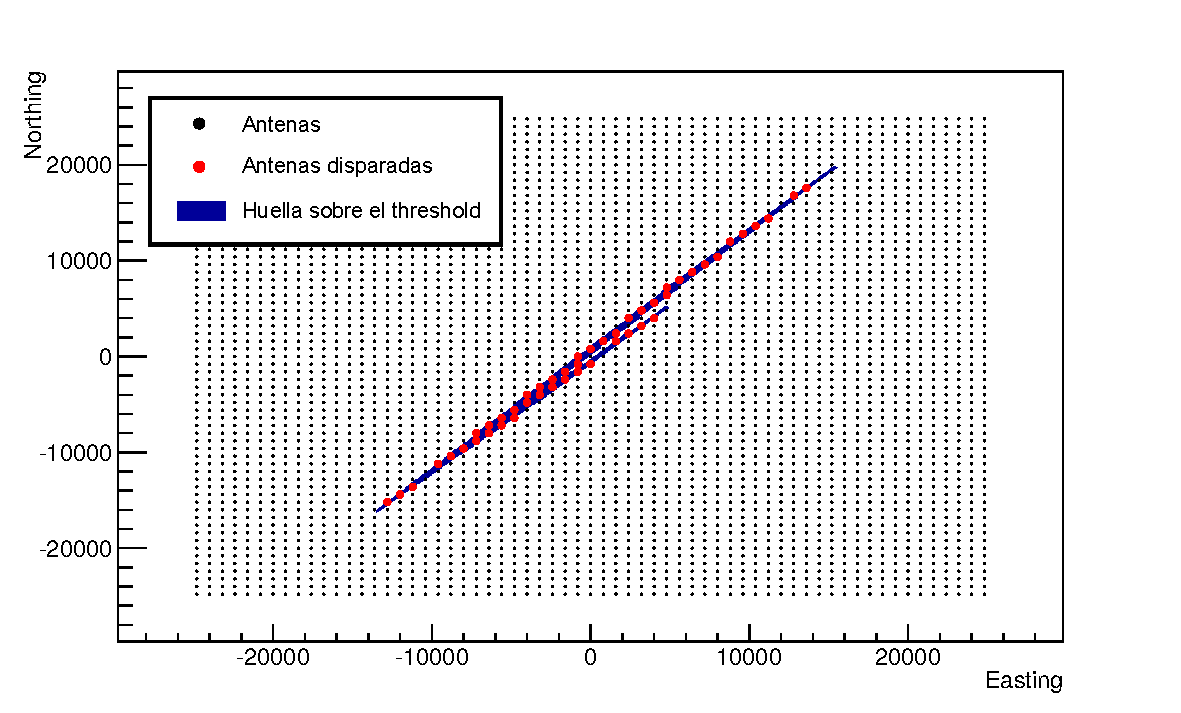
\includegraphics[width=\textwidth]{fig/resultadosRadio/trigger}
			\caption{Evaluaci\'on del disparo global del detector para una lluvia de \cant{E_v=10^{18}}{eV}, $\theta_D=90.5^\circ$ y \cant{{\rm x_d}=25}{m}. Los puntos negros representan las antenas de un arreglo regular de \cant{a_1=a_2=1000}{m} y $\alpha=90^\circ$. En azul se dibuja la regi\'on del suelo en el que la se\~nal super\'o el nivel de disparo local, en este caso \cant{100}{\frac{\mu V}{m}}. En rojo se detallan las antenas pertenecientes al evento.}
			\label{fig:globalTriggerRadio}
		\end{center}
	\end{figure}
	%
	Cada punto negro representa una antena del detector, mientras que la zona azul corresponde al regi\'on en la que la condici\'on de disparo local fue alcanzada, en este caso \cant{100}{\frac{\mu V}{m}}.
	Los puntos rojos marcan las antenas que se consideran parte del evento.
	
	Este procedimiento se llev\'o a cabo para m\'as de 5000 combinaciones de par\'ametros entre las tres topograf\'ias.
	Luego de obtener cada juego de eficiencias de disparo $\varepsilon ({\rm x_d},\theta_D,E_v)$ se descont\'o el canal de decaimiento $\tau^{-}\rightarrow \mu^{-}\bar{\nu_{\mu}}\nu_{\tau}$, que no genera lluvia atmosf\'efica, multiplicando las curvas por $0.826$.
	En la figura \ref{fig:effRadio} se muestra las eficiencias de disparo como funci\'on del \'angulo $\theta_D$ para un detector regular de par\'ametros \cant{a_1=a_2=1500}{m} y $\alpha=60^\circ$, para un nivel de disparo local de \cant{75}{\frac{\mu V}{m}}, para \cant{E_v=\{10^{16.75},10^{17.25},10^{17.75}\}}{eV} y para los valores de \xd{} simulados en cada energ\'ia.
	%
	\begin{figure}[ht!]
		\begin{center}
				\includegraphics[width=0.9\textwidth]{fig/resultadosRadio/eff/{eff50.0_5.0_1000.0_1000.0_60.0_1.0_16.75_m2}.pdf} 
				\includegraphics[width=0.9\textwidth]{fig/resultadosRadio/eff/{eff50.0_5.0_1000.0_1000.0_60.0_1.0_17.25_m2}.pdf}
				\includegraphics[width=0.9\textwidth]{fig/resultadosRadio/eff/{eff50.0_5.0_1000.0_1000.0_60.0_1.0_17.75_m2}.pdf}
			\caption{Curvas de eficiencia como funci\'on del \'angulo cenital obtenidas para un arreglo regular de par\'ametros \cant{a_1=a_2=1500}{m} y $\alpha=60^\circ$, para un nivel de disparo local de \cant{75}{\frac{\mu V}{m}}, para varios valores de \xd{} y para tres valores de energ\'ia visible, \cant{E_v=\{10^{16.75},10^{17.25},10^{17.75}\}}{eV}.}
			\label{fig:effRadio}
		\end{center}
	\end{figure}
	%
	Si bien las curvas de la figura corresponden a un caso particular las siguientes observaciones son generales.
	En primer lugar para cada valor de \xd{} aparece el \'angulo cenital m\'inimo $\theta_D^{cut}$ bajo el cual la eficiencia es 0.
	Adem\'as, de acuerdo con lo discutido en el capitulo \ref{ch:caracterizacionRadio} se cumple:
	\begin{enumerate}
	 \item La eficiencia aumenta al aumentar la energ\'ia visible.
	 \item La eficiencia disminuye al aumentar \xd{}.
	 \item La eficiencia Disminuye al aumentar el \'angulo cenital.
	\end{enumerate}
	
	Otro detalle que resulta notable es que por una peque\~na variaci\'on del \'angulo cenital los eventos pasan de saturar la eficiencia a no conseguir ning\'un disparo del detector.
	
	\clearpage
	\subsection{Eficiencias de identificaci\'on}
	\label{sc:identificacionRadio}
	
	Adem\'as de las eficiencias de disparo, es necesario realizar una estimaci\'on de las eficiencias de identificaci\'on para cada detector.
	Como se expuso en la primer parte de esta tesis, el mayor desaf\'io a la hora de detectar neutrinos ES mediante detectores de superficie resulta ser su discriminaci\'on en el fondo dominante de eventos hadr\'onicos.
	En Auger esto se logra debido a que los tanques \cher{} permiten detectar las lluvias j\'ovenes entre los eventos inclinados, a trav\'es de variables sensibles a la presencia de componente electromagn\'etica.
	En un detector de antenas de radio esta separaci\'on no resulta posible debido a que b\'asicamente toda la emisi\'on es generada proviene de los electrones de media y baja energ\'ia presentes en el m\'aximo de la lluvia.
	Sin embargo la geometr\'ia del cono \cher{} permite salvar este escollo, ya que guarda informaci\'on sobre la ubicaci\'on en la que se produjo dicho m\'aximo, o dicho de otra forma, la t\'ecnica es sensible a la profundidad a la que se inici\'o el evento.
	Para clarificar la situci\'on, en la figura \ref{fig:dg_vs_es_radio} se representa la emisi\'on de un evento hadr\'onico DG inclinado (un evento de background), y uno ES.
	%
	\begin{figure}[ht!]
		\centering
		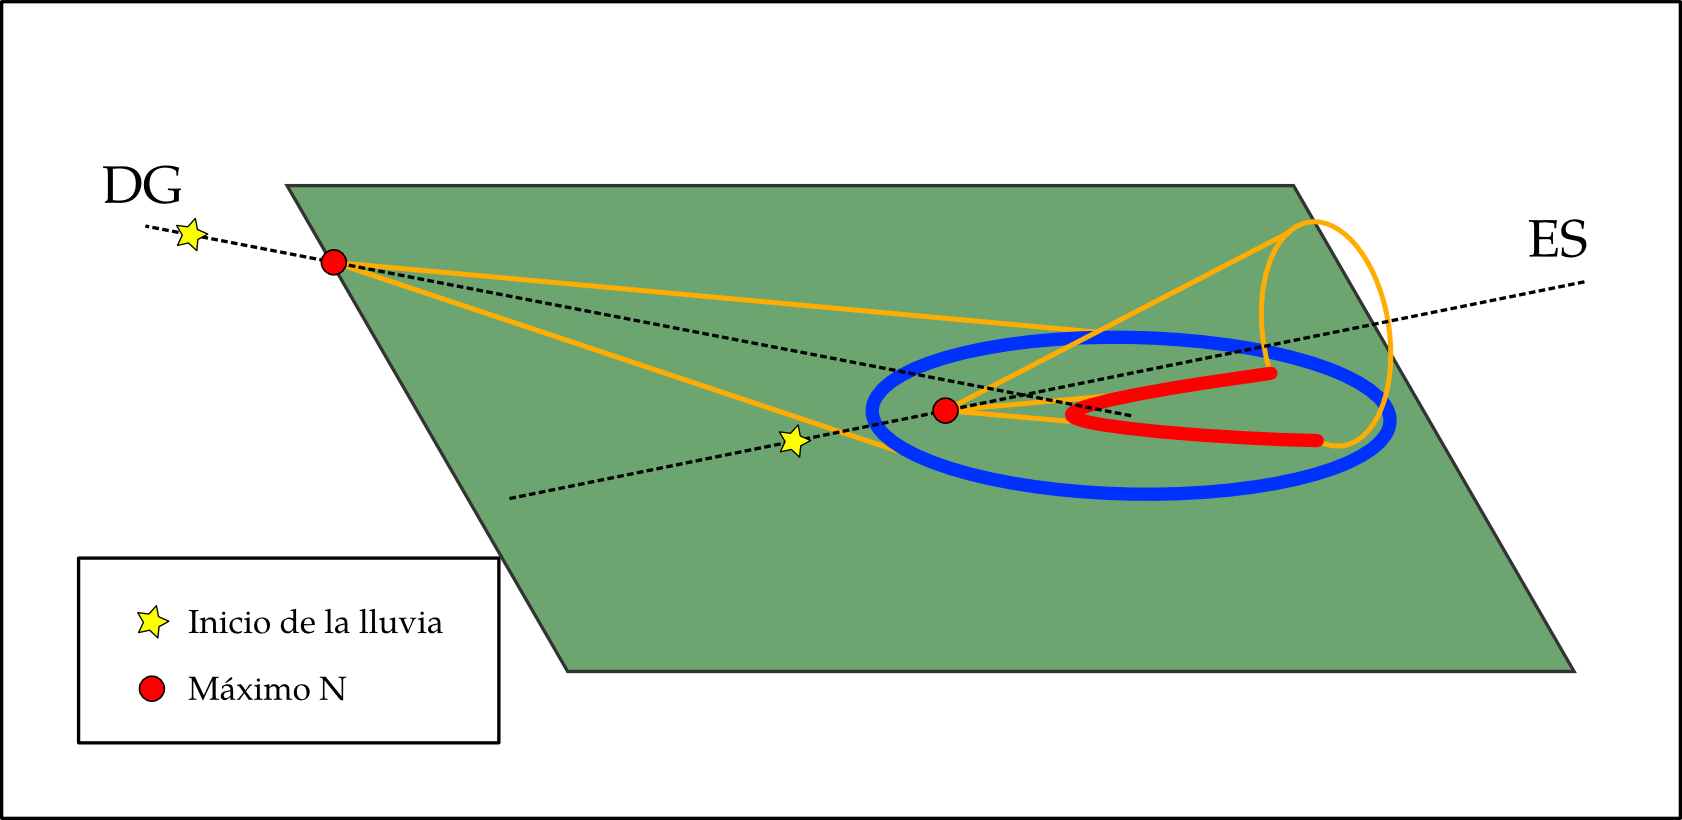
\includegraphics[width=0.8\textwidth]{./fig/simulacionRadio/idRadio.png}
		\caption{\label{fig:dg_vs_es_radio}
		Esquema de las caracter\'isticas que permiten distinguir los eventos ES del fondo de lluvias hadr\'onicas inclinadas (DG). Dado que las lluvias DG se inician alto en la atm\'osfera la apertura del cono \cher{} al nivel de la superficie (l\'inea azul) resulta mucho mayor que la que alcanzar\'ia en un evento ES, debido a que su m\'aximo se produce mucho m\'as cerca de la superficie.
	% 	Adem\'as de la apertura del cono, otro posible factor de discriminaci\'on puede ser la topograf\'ia de la se\~nal a nivel del suelo, ya que en los eventos DG imprimen elipses y los ES hip\'erbolas.
		}
	\end{figure}
	%
	Con esto en mente, la identificaci\'on de eventos ES puede en principio llevarse a cabo a trav\'es de las siguientes diferencias entre las huellas:
	\begin{enumerate}
	 \item La apertura del cono del evento DG a nivel del suelo resulta mayor que la que imprime el evento ES.
	 \item La geometr\'ia de la huella resulta fundamentalmente distinta en los dos casos. En eventos DG es una elipse mientras que en los ES es una hip\'erbola.
	\end{enumerate}

	La primer diferencia proviene de que los eventos hadr\'onicos inclinados se inician cerca del tope de la atm\'osfera, por lo que la emisi\'on debe recorrer distancia mucho mayor que en eventos ES antes de alcanzar el detector.
	De esta manera, el cono \cher{} es cortado por el detector mucho m\'as lejos de su v\'ertice (que resulta ser aproximadamente el m\'aximo de la lluvia), permitiendo una apertura en la huella mucho mayor.
	La segunda diferencia deviene de la forma en la que el detector corta el cono, siendo una elipse en eventos DG y una hip\'erbola en ES.
	Si bien ambas caracter\'isticas tienen potencial de identificaci\'on, la segunda se vuelve m\'as dif\'icil de detectar debido a que en todas las topograf\'ias consideradas la separaci\'on entre antenas es bastante grande y el detalle de la huella suele perderse.
	Por este motivo el resto de esta secci\'on busca determinar la factibilidad de la identificaci\'on basado en la medici\'on de la apertura de la huella.
	
	Hasta el momento lo expuesto es una conjetura basada en la intuici\'on anada en el estudio de los resultados del cap\'itulo \ref{ch:caracterizacionRadio}.
	Para sostenerla se realizaron simulaciones de eventos DG, que se muestran en la figura \ref{fig:dg_thetas}, 
	%
	\begin{figure}[ht!]
		\centering
		\begin{tabular}{cc}
		$\theta_D=85^\circ$ & $\theta_D=87^\circ$ \\
		\includegraphics[width=0.5\textwidth]{./fig/resultadosRadio/dg/{foorPrint_ZWv1.33_ntuples_v1.22_Downgoing_phi_90_19.5_85_90_100_1_E}.pdf} &
		\includegraphics[width=0.5\textwidth]{./fig/resultadosRadio/dg/{foorPrint_ZWv1.33_ntuples_v1.22_Downgoing_phi_90_18.5_87_90_100_2_E}.pdf}\\
		
		$\theta_D=88^\circ$ & $\theta_D=89^\circ$ \\
		\includegraphics[width=0.5\textwidth]{./fig/resultadosRadio/dg/{foorPrint_ZWv1.33_ntuples_v1.22_Downgoing_phi_90_18.5_88_90_100_6_E}.pdf} &
		\includegraphics[width=0.5\textwidth]{./fig/resultadosRadio/dg/{foorPrint_ZWv1.34_ntuples_v1.22_Downgoing_phi_90_18.5_89_90_100_5_E}.pdf}\\
		\end{tabular}
		\caption{\label{fig:dg_thetas}
		Huella sobre el detector para eventos DG de $\theta_D=\{85^\circ,87^\circ,88^\circ,89^\circ\}$. De acuerdo con lo esperado, su tama\~no en la direcci\'on transversal resulta sustancialmente mayor que en eventos ES. 
		}
	\end{figure}
	%
	donde se expone la huella dejada por un evento iniciado por un proton de \cant{10^{18}}{eV} a una profundidad de \cant{200}{g/cm^2}, y con $\theta_D=\{85^\circ,87^\circ,88^\circ,89^\circ\}$.
	Tal como se hab\'ia supuesto la geometr\'ia de la huella es fundamentalmente distinta a la de los eventos ES.
	En primer lugar su largo crece a medida que el \'angulo aumenta, pasando de \cant{\sim40}{km} a $85^\circ$ hasta casi \cant{300}{km} $89^\circ$.
	Por otro lado el ancho var\'ia entre \cant{4000}{m} a \cant{8000}{m} lo que supera el observado en eventos ES, que ronda los \cant{2000}{m} (ver cap\'itulo \ref{ch:caracterizacionRadio}).
	
% 	Esto se debe a que el m\'aximo ocurre en todos los casos aproximadamente a la misma profundidad \cant{\sim 1000}{g/cm^2}, que se aleja del detector a medida que \td{} crece.
	
	Para estudiar con detalle la eficiencia de identificaci\'on se deber\'ian realizar por lo menos algunos cientos de simulaciones de eventos DG. 
	Al iniciarse cerca del tope de la atm\'osfera el volumen de simulaci\'on de \aires{} resulta inmenso, lo que implica el seguimiento de las part\'iculas durante mucho m\'as tiempo de simulaci\'on, calculando en cada avance la se\~nal en todas las antenas.
	Esto implica que este tipo de eventos requieran mucho m\'as tiempo de CPU que los eventos ES.
	En particular, para obtener las lluvias que se muestran en la figura \ref{fig:dg_thetas} se utiliz\'o del orden de 300 dias de CPU para cada una, lo que vuelve el estudio detallado impracticable con los recursos disponibles.
	Como alternativa, en la figura \ref{fig:dg_vs_es_Idradio} se muestra el ancho promedio de la huella calculado sobre el detector denso para toda la muestra de eventos ES y DG.
	En acuerdo con lo expuesto hasta el momento se observa que los eventos DG muestran un ancho mayor que los eventos ES.
	En base a esta caracter\'istica es posible presumir que la identificaci\'on de eventos ES no s\'olo es factible sino que ser\'a adem\'as eficiente.
	Para calcular la exposici\'on entonces se supondr\'a una eficiencia de identificaci\'on entre 0.8 y 1\footnote{Estos n\'umeros son razonables si se tiene en cuenta que la eficiencia de identificaci\'on de neutrinos ES en Auger supera el 90$\%$.}.
	%
	\begin{figure}[ht!]
		\centering
		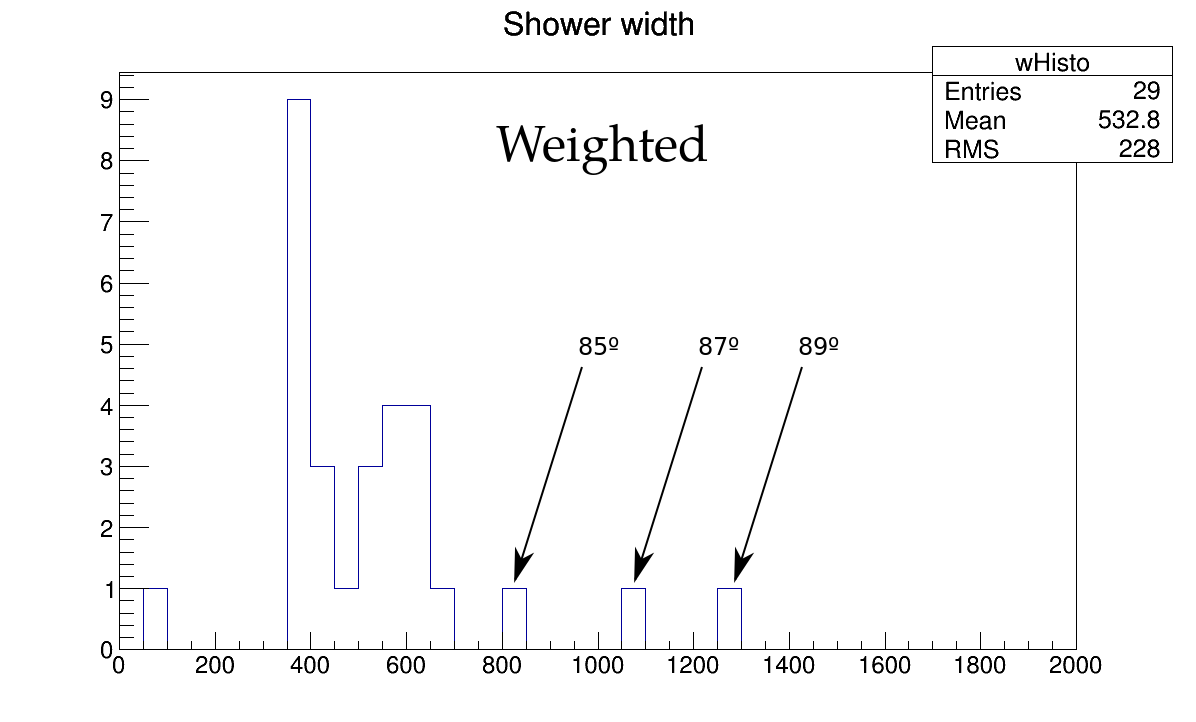
\includegraphics[width=\textwidth]{./fig/resultadosRadio/showerWidth_Comp_DG_ES_Wt}
		\caption{\label{fig:dg_vs_es_Idradio}
		Separaci\'on en el ancho de la lluvia de eventos DG y ES. 
		}
	\end{figure}
	
	% 
	% 
	% Tambi\'en, se nota como la opograf\'ia de la huella en ambos casos es fundamentalmente distinta, ya que el evento DG imprime una elipse sobre el suelo y el evento ES una hip\'erbola.
	% En consecuencia se estudiar\'a si es posible explotar estas diferencias para identificar eventos ES.

% 	Por otra parte, en la figura 

% 	- eventos gigantes

% 	- se inician lejos y el campo cae como 1/R pero el drift es mayor debido a la baja densidad de la atm\'osfera

% 	- ver v4.20 en ntuple analizer mostrar que la velocidad sobre el eje y el ancho 

% \subsubsection{Resumen del an\'alisis de la se\~nal}
% 
% 	\begin{table}[ht!]
% 	\centering
% 	\begin{tabular}{|p{0.3\textwidth}|p{0.7\textwidth}|}
% 	\toprule
% 	Descripci\'on & Detalle \\
% 	\midrule\midrule
% 	Filtrado de la se\~nal & Respuesta plana en la banda \cant{30\text{-}80\text{/}120\text{-}900}{MHz} \\ \midrule
% 	Nivel de disparo local &  Entre \cant{25}{\frac{\mu V}{m}} y \cant{200}{\frac{\mu V}{m}} con un paso de \cant{25}{\frac{\mu V}{m}}\\ \midrule
% 	Disparo global & Antenas disparadas compatibles con un frente que se desplaza a la velocidad de la luz \\ \midrule
%  	Nivel de identificaci\'on & Eficiencia entre 0.80 y 1.00 con un paso de 0.05 \\
% 	
% 	\bottomrule
% 	\end{tabular}
% 	\end{table}

	
\section{Desempe\~no de un detector de 90000 antenas}
	
	El objetivo de la segunda parte de esta tesis es estimar el desempe\~no de un detector de superficie de 90000 antenas de radio, y es a lo que se dedica esta secci\'on.
	En esta l\'inea una vez definidos los criterios y m\'etodos que permiten calcular las eficiencias de detecci\'on es posible en primer lugar estudiar qu\'e aspectos del dise\~no son relevantes, determinando cu\'anto impacta cada uno sobre la medici\'on.
	Al mismo tiempo se utiliz\'o toda la informaci\'on recolectada haste el momento, junto con la ecuaci\'on \ref{eq:exp2ESRadio}, para obtener l\'imites diferenciales al 90$\%$ de nivel de confianza que podr\'ia imponer el detector y se lo comparar\'a con la proxima generaci\'on de detectores de neutrinos.
	Por \'ultimo se analiza en el marco de los modelos vigentes en la actualidad, cu\'antos eventos se esperan medir con este tipo de detectores en un per\'iodo de 3 a\~nos.
	
	\subsection{Aspectos del dise\~no}
	
	En los cap\'itulos \ref{ch:simulacionRadio} y \ref{ch:caracterizacionRadio} se utiliz\'o informaci\'on recavada sobre la emisi\'on de radio de cascadas atmosf\'ericas para, entre otras cosas, acotar las caracter\'isticas de dise\~no del detector.
	Sin embargo, existen ciertas caracter\'isticas que no se encuentran completamente determinadas, a saber:
	%
	\begin{enumerate}
	 \item La topograf\'ia del detector;
	 \item Su extensi\'on;
	 \item El nivel de disparo local;
	 \item Las caracter\'isticas del disparo global.
	\end{enumerate}
	
	Dado que el objetivo es detectar neutrinos, la variable natural para evaluar la bondad de cada configuraci\'on es el n\'umero de eventos esperado durante una medici\'on, hipot\'etica a este nivel.
	Recordando la ecuaci\'on \ref{eq:exp1} del cap\'itulo \ref{ch:expAuger}, esta cantidad puede obtenerse mediante:
	%
	\begin{equation}
		N_{Radio} = \int\limits_{\mathbf{E_\nu}}~\Phi(E_{\nu})~\mathcal{E}(E_\nu)~dE_{\nu}
		\label{eq:nesp_radio}
	\end{equation}
	%
	Para llevar a cabo las comparaciones salvo que se indique lo contrario se utilizar\'a un escenario $\Phi(E_{\nu})\sim E_{\nu}^{-2}$ y $\mathcal{E}(E_\nu)$ ser\'a calculada mediante la ecuaci\'on \ref{eq:exp2ESRadio}.
	Adem\'as, con el fin de enmarcar el resultado se informar\'a esta cantidad en unidades de $N_{Auger}$ (o sea $N_{Radio}/N_{Auger}$), que representa los eventos ES que detectar\'ia el SD Auger en una medici\'on equivalente\footnote{Mismo flujo y misma duraci\'on. No mismo tama\~no.}.
	
	Por otro lado ser\'a interesante estudiar el comportamiento del argumento de la integral \ref{eq:nesp_radio}, que contiene informaci\'on sobre la sensitividad del detector a diferentes energ\'ias.
	Para simplificar la comparaci\'on entre la abultada cantidad de configuraciones estudiadas, se decidi\'o utilizar como medida de la sensibilidad la energ\'ia media esperada en los neutrinos detectados, dada por:
	%
	\begin{equation}
		\langle E_{\nu}\rangle = \int\limits_{\mathbf{E_\nu}}~E_\nu~\Phi(E_{\nu})~\mathcal{E}(E_\nu)~dE_{\nu}
		\label{eq:emean_radio}
	\end{equation}
	
	A partir de aqu\'i entonces se estudiar\'an estas cantidades como funci\'on de los distintos par\'ametros todav\'ia libres en el dise\~no del detector.
	
	\subsubsection{Topograf\'ias y niveles de disparo}
	
	La topograf\'ia del detector de tipo regular (RE) y panal de abeja (HC, por \emph{honeycomb}) queda definida por los par\'ametros $\left\{a_1,a_2,\alpha\right\}$ mientras que en la de bordes densos (DE, por \emph{dense edge}) por el conjunto $\left\{d,D\right\}$.
	Sin embargo, debido a que en topograf\'ias RE y HC las configuraciones con $a_1$ muy distinto de $a_2$ (dentro de valores razonables) pueden lograrse aproximadamente imponiendo $a_1=a_2$ y un valor adecuado para $\alpha$, con el fin de acotar el n\'umero de configuraciones consideradas s\'olo se estudiaron casos en los que se cumple la condici\'on $a_1=a_2$.
	Entonces en todas las topograf\'ias (RE, HC y DE) bast\'o dar 2 n\'umeros para determinar completamente la disposici\'on de antenas sobre la superficie del detector.
	
	Adem\'as de los par\'ametros que determinan la configuraci\'on, para poder comparar las cantidades $N_{Radio}$ y $N_{Auger}$ de manera justa fue necesario calcular sus valores en tiempos de medici\'on equivalentes e incluir la diferencia de tama\~no relativa entre los detectores.
	Para conciliar en primer lugar el tiempo de medici\'on se calcul\'o $N_{Radio}$ imponiendo \cant{T=1}{s} en la ecuaci\'on \ref{eq:exp2ESRadio} mientras que $N_{Auger}$ fue calculado utilzando la exposici\'on \emph{Full Auger} a neutrinos ES para \cant{6.5}{yr} y se la dividi\'o por \cant{2.05\times10^8}{s}~\footnote{Este n\'umero corresponde a 6.5 a\~nos en segundos.}, obteniendo de esa manera la exposici\'on promedio por segundo del observatorio.
	Luego, para incluir la diferencia de tama\~no de los detectores en cada configuraci\'on se determin\'o la celda primitiva correspondiente, se calcu\'o su \'area y el n\'umero de celdas que completan el arreglo, para al fin calcular la superficie cubierta en cada caso.
	
	Para el SD de Auger por ejemplo la superficie de la celda primitiva se puede calcular como \cant{1500^2\sin60^\circ}{m^2}=\cant{1.94\times10^6}{m^2}, y cada una contiene una sola estaci\'on.
	Entonces, dado que el detector completo esta conformado por 1600 de estas celdas la superficie total cubierta es de \cant{1600\times1.94\times10^6}{m^2}$\sim$\cant{3100}{km^2}.
	Por otra parte, un detector de radio con la misma configuraci\'on, \cant{a_1=a_2=1500}{m} y $\alpha=60^\circ$, y 90000 celdas primitivas posee una superficie cubierta de \cant{90000\times1.94\times10^6}{m^2}$\sim$\cant{174000}{km^2}.
	Por ende, en este caso particular el n\'umero de eventos extra debido a la diferencia de superficie instrumentada es de alrededor de $56.25$ m\'as a favor del detector de radio.
	
	Si en vez de un areglo regular se considera uno tipo panal de abeja, con \cant{a_1=a_2=1500}{m} y $\alpha=60^\circ$, la cuenta es levemente diferente. 
	En este caso en lugar de utilizar la celda de Wigner-Seitz, que se grafica en la figura \ref{fig:corePos2} y cuya expresi\'on en es poco intuitiva, es posible explotar el hecho de que un arrego HC es uno RE en el que se quita un nodo cada tres.
	Entonces es posible pensar que cada celda primitiva, de \'area \cant{1.94\times10^6}{m^2}, utiliza s\'olo $2/3$ de antena, o lo que es lo mismo, que el \'area total cubierta ser\'a $3/2$ la de un arreglo regular equivalente.
	Finalmente, para calcular la celda primitiva de un arreglo de bordes densos, dado que s\'olo se consideraron configuraciones en las que $D/d\epsilon\mathbb{N}$, se tiene que el \'area de la celda es $D^2$, mientras que la cantidad de antenas necesarias para construir cada una es $2\frac{D}{d}-1$. 
	Por este motivo la superficie total cubierta por un detector de 90000 antenas ser\'a $\frac{90000}{2\frac{D}{d}-1}\times D^2$.
	Todo esto se resume en la tabla \ref{tab:conv2Auger}, que detalla para cada familia de topograf\'ias y para el SD de Auger el \'area de la celda primitiva, cu\'antas antenas se requieren para conformarla y el n\'umero de celdas que forman al detector.
	\begin{table}
	\centering
	\renewcommand{\arraystretch}{2.5}
	\footnotesize
	\begin{tabular}{lccc}
	\hline
	 Topograf\'ia & \'Area cubierta por celda  & Antenas por celda & N\'umero de celdas \\
	\hline
	 Auger &\cant{1.94\ 10^6}{m^2}&1&1600\\
	 Regular &\multirow{2}{*}{$a_1a_2\sin\alpha$}&1&90000\\
	 Panal de abeja &&$\frac{2}{3}$&$90000\frac{3}{2}$\\
	 Bordes densos &$D^2$&$\frac{2D}{d}-1$& $\dfrac{90000}{\frac{2D}{d}-1}$\\[0.3cm] \hline
	\end{tabular}
	\caption{\label{tab:conv2Auger} Factores necesarios para calcular la superficie cubierta por un detector con una dada topograf\'ia. En el arreglo de bordes densos se utiliz\'o como restricci\'on que $\frac{D}{d}\,\epsilon\,\mathbb{N}$. Finalmente la superficie se calcula multiplicando el \'area por celda por el n\'umero total de celdas dadas 90000 antenas.
	}
	\end{table}
	%
	
	En estas condiciones las figuras \ref{fig:compRadioAuger_re}, \ref{fig:compRadioAuger_hc} y \ref{fig:compRadioAuger_de}, muestan $N_{Radio}/N_{Auger}$ para diferentes combinaciones de par\'ametros simuladas, para las topograf\'ias RE, HC y DE respectivamente. 
	En los tres casos como nivel de disparo local se utiliz\'o \cant{50}{\mu V/m}, como disparo global 5 antenas disparadas (aOT) y un nivel de identificaci\'on hipot\'etico de $90\%$.
	%
	\begin{figure}[h!]
		\begin{center}
			\textbf{\footnotesize Arreglo regular}\\
			\includegraphics[width=\textwidth]{fig/resultadosRadio/perf/param/{CompRadioAuger_50.0_5.0_1.0_re_modo1}.pdf}
			\caption{\label{fig:compRadioAuger_re} Relaci\'on entre los eventos esperados en un detector regular de par\'ametros $a_1=a_2$ y $\alpha$ para algunos de las combinaciones estudiadas. Como nivel de disparo local se utiliz\'o \cant{50}{\mu V/m}, se pidieron al menos 5 antenas disparadas por evento y un nivel de identificaci\'on hipot\'etico de $90\%$.}
		\end{center}
	\end{figure}
	%
	\begin{figure}[h!]
		\begin{center}
			\textbf{\footnotesize Arreglo tipo panal de abeja}\\
			\includegraphics[width=\textwidth]{fig/resultadosRadio/perf/param/{CompRadioAuger_50.0_5.0_1.0_hc_modo1}.pdf}
			\caption{\label{fig:compRadioAuger_hc} Relaci\'on entre los eventos esperados en un detector tipo panal de abeja de par\'ametros $a_1=a_2$ y $\alpha$ para algunos de las combinaciones estudiadas. Como nivel de disparo local se utiliz\'o \cant{50}{\mu V/m}, se pidieron al menos 5 antenas disparadas por evento y un nivel de identificaci\'on hipot\'etico de $90\%$.}
		\end{center}
	\end{figure}
	%
	\begin{figure}[h!]
		\begin{center}
			\textbf{\footnotesize Arreglo de bordes densos}\\
			\includegraphics[width=\textwidth]{fig/resultadosRadio/perf/param/{CompRadioAuger_50.0_5.0_1.0_de_modo2}.pdf}
			\caption{\label{fig:compRadioAuger_de} Relaci\'on entre los eventos esperados en un detector de bordes densos de par\'ametros $d$ y $D$ para algunos de las combinaciones estudiadas. Como nivel de disparo local se utiliz\'o \cant{50}{\mu V/m}, se pidieron al menos 5 antenas disparadas por evento y un nivel de identificaci\'on hipot\'etico de $90\%$.}
		\end{center}
	\end{figure}
	%
	
	La primer observaci\'on en la figura \ref{fig:compRadioAuger_re} es que para un arreglo de radio de las caracter\'isticas de Auger (\cant{a_1=a_2=1500}{m} y $\alpha=60^\circ$) se esperaba en principio, una ganancia de $56.25$ debido al incremento de superficie y una p\'erdida del \'orden de un factor $3$ debido a la diferencia de rango angular observado (ver figura \ref{fig:gainThetas}), con lo que se esperar\'ia que el detector de radio detecte del orden de $56.25/3\sim19$ veces m\'as eventos que Auger. 
	Sin embargo para estos valores de threshold local y global la relaci\'on observada es un factor $\sim100$~\footnote{El valor debe ser estimado interpolando, para $60^\circ$, los puntos amarillo y el naranja.}.
	Esto quiere decir que en estas condiciones el arreglo de radio es m\'as eficiente a baja energ\'ia, el \'unico lugar del que puede provenir el exceso de eventos observado.
	
	Para analizar ahora el impacto de cada uno de los par\'ametros en el cociente de eventos es fundamental comprender c\'omo puede afectar un cambio en la topograf\'ia a la exposici\'on del detector. En esta l\'inea a grandes rasgos es posible aislar dos efectos que compiten entre s\'i:
	%
	\begin{enumerate}
	 \item Una disminuci\'on en la granularidad provocar\'a un aumento en la superficie total instrumentada, lo que aumenta la exposici\'on.
	 \item Un aumento en la granularidad elevar\'a las eficiencias a baja energ\'ia, lo que en un escenario $E_\nu^{-2}$ elevar\'a la exposici\'on.
	\end{enumerate}
	%
	Sin embargo el detalle de la topograf\'ia, es decir c\'omo es la distribuci\'on particular de antenas dentro de cada celda primitiva, podr\'ia en principio compensar o profundizar cualquiera de los dos efectos\footnote{Supongamos una celda primitiva de 10 antenas y \cant{10}{km^2} de superficie efectiva. Si bien el \'area total cubierta de un detector conformado por estas celdas ser\'ia siempre la misma (\cant{90000}{km^2} en nuestro detector), la eficiencia se ver\'a modificada si todas las antenas estan aglomeradas en un punto o si se encuentran equidistribuidas a trav\'es de los \cant{10}{km^2}.}.
	
	Entonces, con esto en mente es posible analizar los resultados mostrados en las figuras, donde pueden ser aisladas algunas caracter\'isticas interesantes.
	En las topograf\'ias RE y HC (figuras \ref{fig:compRadioAuger_re} y \ref{fig:compRadioAuger_hc}) la cantidad de eventos esperados aumenta con el \'angulo $\alpha$ y al aumentar los pasos $a_1$ y $a_2$.
	Esto quiere decir que al menos en estas condiciones de disparo local y global los t\'erminos $a_1 \times a_2$ y $\sin \alpha$ en el c\'alculo de la superficie cubierta por el detector se imponen por sobre la p\'erdida de eficiencia que podr\'ia provocar la separaci\'on de las antenas.
	De igual forma, en la topograf\'ia DE (figura \ref{fig:compRadioAuger_de}) los par\'ametros el n\'umero de eventos esperados aumenta con $d$ y $D$, lo que indica nuevamente que el incremento en el \'area termina imponiendose por sobre la p\'erdida de eficiciencia.
	En ambos casos lo que sucede es que el nivel de disparo local de las antenas elegido es lo suficientemente bajo como para que incluso a baja energ\'ia la huella de los eventos por encima de ese nivel sea lo suficientemente extensa para disparar al menos 5 antenas.
	Esto no es siempre de esta manera, por ejemplo en la figura \label{fig:compRadioAuger_th2} se muestra la cantidad de eventos como funci\'on de los pasos $a_1$ y $a_2$ para varios valores de $\alpha$ en un arreglo regular, para un threshold local de \cant{100}{\mu V/m} y uno global de 9 antenas.
	%
	\begin{figure}[h!]
		\begin{center}
			\textbf{\footnotesize Arreglo regular}\\
			\includegraphics[width=\textwidth]{fig/resultadosRadio/perf/sat/{CompRadioAuger_100.0_9.0_1.0_hc_modo2}.pdf}
			\caption{\label{fig:compRadioAuger_th2} Eventos esperados como funci\'on del paso $a_1,a_2$ en un detector tipo regular, para varios valores de $\alpha$. Como nivel de disparo local se utiliz\'o \cant{100}{\mu V/m}, se pidieron al menos 9 antenas disparadas por evento y un nivel de identificaci\'on hipot\'etico de $90\%$. Para $\alpha=90^\circ$ y $\alpha=60^\circ$ existe un valor de $a_1,a_2$ en el que la p\'erdida de eficiencia a baja energ\'ia supera la ganancia de superficie.}
		\end{center}
	\end{figure}
	%
	Este aumento en el nivel de umbral de disparo local implica que el tama\~no de la huella por encima del mismo disminuya~\footnote{Esto puede corroborarse a simple vista en cualquiera de las figuras de la huella del detector del cap\'itulo \ref{ch:caracterizacionRadio}.}, lo que dificulta que se cumpla la condicion de disparo global ($n$ cantidad de antenas disparadas).
	Entonces si se considera en la figura por ejemplo la curva marr\'on, que corresponde a $\alpha=90^\circ$, puede notarse c\'omo a partir de \cant{a_1,a_2 = 1400}{m} la p\'erdida de eventos de baja energ\'ia supera el aumento del \'area que implica el incremento del paso del detector.
	Lo mismo sucede para $\alpha=60^\circ$ (curva verde) y \cant{a_1,a_2 = 1600}{m}.
	
	Para generalizar esta idea las figuras \ref{fig:compRadioAuger_th} y \ref{fig:compRadioAuger_th2} muestran c\'omo cambia la cantidad de eventos esperados y el valor medio de la energ\'ia (calculado con la ecuaci\'on \ref{eq:emean_radio}) en funci\'on del threshold local, para varios valores de $D$ en un arreglo tipo DE.
	%
	\begin{figure}[h!]
		\begin{center}
			\textbf{\footnotesize Arreglo de bordes densos}\\
			\includegraphics[width=\textwidth]{fig/resultadosRadio/perf/thresh/{CompRadioAuger_1000.0_5.0_1.0_de_modo3}.pdf}
			\caption{\label{fig:compRadioAuger_th} Numero de eventos esperados como funci\'on del nivel de disparo local y para distintos valores de $D$ en un arreglod e bordes densos. Se observa un decaimiento a medida que aumenta el threshold.}
		\end{center}
	\end{figure}
	%
	\begin{figure}[h!]
		\begin{center}
			\textbf{\footnotesize Arreglo de bordes densos}\\
			\includegraphics[width=\textwidth]{fig/resultadosRadio/perf/ener/{CompRadioAuger_1000.0_5.0_1.0_de_modo4}.pdf}
			\caption{\label{fig:compRadioAuger_th3} Valor medio de la energ\'ia seg\'un la ecuaci\'on \ref{eq:emean_radio} como funci\'on del threshold local para varios valores de $D$ en un arreglo de bordes densos. Se observa que la energ\'ia media aumenta con el valor del treshold para todos los valores de $D$. Esto es consistente con la p\'erdida de eventos de baja energ\'ia.}
		\end{center}
	\end{figure}
	%
	Se observa en la figura \ref{fig:compRadioAuger_th} como para cada valor de $D$ un aumento de threshold disminuye la cantidad de eventos esperados mientras que al mismo tiempo, en la figura \ref{fig:compRadioAuger_th3} el valor medio de la energ\'ia aumenta.
	Este comportamiento implica una p\'erdida relativa de eventos de baja energ\'ia.
	
	Para estudiar entonces el comportamiento del detector cerca de sus l\'imites de nivel de ruido (ver secci\'on \ref{sbsc:localTriggerRadio}) a partir de aqu\'i se fijar\'a el nivel de disparo local en \cant{50}{\mu V/m} y se exigir\'a una condici\'on de disparo global de al menos 5 detectores disparados, lo m\'inimo razonable para realizar una reconstrucci\'on geom\'etrica confiable.
	Bajo estas condiciones la premisa para aumentar la exposici\'on del detector es aumentar el \'area al m\'aximo posible, lo que introduce la siguiente secci\'on.
	
	\subsubsection{Limitaci\'on en extensi\'on}
	
	En la actualidad el SD m\'as extenso es el del Observatorio Pierre Auger, cubriendo una superficie de \cant{\sim3000}{km^2} se encuentra desplegado en una regi\'on de aproximadamente \cant{50}{km} $\times$ \cant{50}{km}. 
	Por otra parte, el proyecto GRAND propone instalar las 90000 antenas en un arreglo cuadrado de \cant{800}{m} de paso, lo que supone un \'area instrumentada de \cant{\sim60000}{km^2} en una regi\'on de \cant{\sim250}{km} de lado~\footnote{El tama\~no de la provincia de Jujuy!}. 
	A esta escala la dimensi\'on del detector pasa a ser un factor limitante debido a factores como por ejemplo el costo de operaci\'on, de mantenimiento o simplemente no es posible encontrar un lugar donde ubicarlo. 
	Esto implica que, dado un n\'umero fijo de antenas, no cualquier combinaci\'on de par\'ametros del conjunto simulado es viable como un experimento real.
	Entonces para encarar esta cuestion se calcul\'o para las tres topograf\'ias la superficie cubierta $S$ por cada detector simulado y la \emph{dimensi\'on equivalente} $L=\sqrt{S}$, que corresponde al lado de un detector cuadrado que cubre tal superficie.
	En la figura \ref{fig:compRadioAuger_area0} se muestra a modo de ejemplo $L$ como funci\'on de los par\'ametros $a_1=a_2$ y $\alpha$ par aun arreglo regular.
	%
	\begin{figure}[h!]
		\begin{center}
			\includegraphics[width=\textwidth]{fig/resultadosRadio/perf/area/{Area_re}.pdf}
			\caption{\label{fig:compRadioAuger_area0} Lado equivalente de un SD cuadrado de topograf\'ia regular como funci\'on de los par\'ametros $a_1=a_2$ y $\alpha$. En l\'ineas negras se marca el valor de $L$ correspondiente a GRAND, \cant{250}{km}, y el considerado como m\'aximo razonable en esta tesis, \cant{500}{km}.}
		\end{center}
	\end{figure}
	%
	En l\'ineas negras se resalta la dimensi\'on equivalente de GRAND, y lo que aqu\'i se considerar\'o como la m\'axima extensi\'on viable para la t\'ecnica, \cant{500}{km}.
	Luego con esta informaci\'on fue posible determinar cuales de las topograf\'ias simuladas pueden ser consideradas viables en este sentido o no.
	Entonces en las figuras \ref{fig:compRadioAuger_area_re}, \ref{fig:compRadioAuger_area_hc} y \ref{fig:compRadioAuger_area_de} se resaltan las configuraciones v\'alidas en las tres topograf\'ias, es decir, los casos que cumplen \cant{L<500}{km} y \cant{L<250}{km}.
	%
	\begin{figure}[h!]
		\begin{center}
			\textbf{\footnotesize Arreglo regular}\\
			\includegraphics[width=\textwidth]{fig/resultadosRadio/perf/area/{CompRadioAuger_50.0_5.0_1.0_re_modo1}.pdf}
			\caption{\label{fig:compRadioAuger_area_re} Se resalta en la figura \ref{fig:compRadioAuger_re} las configuraciones que poseen un valor de \cant{L<500}{km} y \cant{L<250}{km}.}
		\end{center}
	\end{figure}
	%
	\begin{figure}[h!]
		\begin{center}
			\textbf{\footnotesize Arreglo tipo panal de abeja}\\
			\includegraphics[width=\textwidth]{fig/resultadosRadio/perf/area/{CompRadioAuger_50.0_5.0_1.0_hc_modo1}.pdf}
			\caption{\label{fig:compRadioAuger_area_hc} Se resalta en la figura \ref{fig:compRadioAuger_hc} las configuraciones que poseen un valor de \cant{L<500}{km} y \cant{L<250}{km}.}
		\end{center}
	\end{figure}
	%
	\begin{figure}[h!]
		\begin{center}
			\textbf{\footnotesize Arreglo de bordes densos}\\
			\includegraphics[width=\textwidth]{fig/resultadosRadio/perf/area/{CompRadioAuger_50.0_5.0_1.0_de_modo2}.pdf}
			\caption{\label{fig:compRadioAuger_area_de} Se resalta en la figura \ref{fig:compRadioAuger_re} las configuraciones que poseen un valor de \cant{L<500}{km} y \cant{L<250}{km}.}
		\end{center}
	\end{figure}
	%
	Se observa que el m\'aximo desempe\~no alcanzado por el detector cuando \cant{L<250}{km} se encuentra cercano a 40 en las tres topograf\'ias, mientras que el logrado cuando \cant{L<500}{km} ronda los 150.
	Si bien en el arreglo RE estos valores m\'aximos parecen ser levemente menores que en los casos HC y DE, a primer orden y para estos niveles de disparo la topograf\'ia no es un factor determinante del desempe\~no del detector.
	Todo lo expuesto hasta el momento indica que la cantidad esperada de eventos crece significativamente con la superficie cubierta por el detector.
	Por otra parte es muy probable que la calidad de los eventos detectados por arreglos RE, HC y DE presenten s\'i diferencias significativas, pero este tema no fue abordado en esta tesis~\footnote{En particular la topograf\'ia DE fue ideada con el fin de mejorar la calidad de los eventos detectados, bajo la premisa de aprovechar las dos dimensiones que muestran este tipo de lluvias. Ante un evento sobre cada borde de las celdas se disparar\'ian peque\~nos clusters de antenas, lo que permitir\'ia en principio mejorar significativamente la reconstrucci\'on de las variables geom\'etricas.}.
	
	Entonces para analizar el desempe\~no del detector, que es a lo que se dedica la siguiente secci\'on, se utiliz\'o en el c\'alculo de la exposici\'on de cada topograf\'ia la combinaci\'on de par\'ametros simulada que arroj\'o la mayor cantidad de eventos esperados luego de aplicar las condiciones \cant{L<500}{km} y \cant{L<250}{km}, lo que se detalla en la tabla \ref{tab:bestConf}.
	
	\begin{table}[ht!]
	\begin{center}
	\renewcommand{\arraystretch}{2}
	\small
		\begin{tabular}{|l|cc|cc|cc|}
			\hline
			\multirow{3}{*}{Condici\'on} & \multicolumn{6}{c|}{Topograf\'ia} \\
			&  \multicolumn{2}{c}{Regular} & \multicolumn{2}{c}{Panal de abeja} &   \multicolumn{2}{c|}{Bordes densos} \\ \cline{2-7}
			& $a_1,a_2$ & $\alpha$& $a_1,a_2$ & $\alpha$& $d$ & $D$\\
			\hline
			\cant{L<500}{km} &\cant{2000}{m}&$90^\circ$&\cant{2000}{m}&$30^\circ$&\cant{750}{m}&\cant{7500}{m} \\
			\cant{L<250}{km}  &\cant{1600}{m}&$15^\circ$&\cant{1400}{m}&$15^\circ$&\cant{250}{m}&\cant{6000}{m}  \\
			\hline
		\end{tabular}
		\caption{\label{tab:bestConf} Configuraciones simuladas que arrojan mayor cantidad de eventos esperados bajo las condiciones \cant{L<500}{km} y \cant{L<250}{km} para cada una de las topograf\'ias.}
	\end{center}
	\end{table}
	
	\subsection{Perspectivas de la t\'ecnica}
	
	Una vez definido los detectores representativos de cada topograf\'ia y calculadas sus exposiciones, es necesario estudiar c\'omo se posiciona cada uno de ellos en la proxima generaci\'on de detectores de neutrinos ultra energ\'eticos.
	Para ello, siguiendo el procedimiento descripto en la secci\'on \ref{sc:limiteAuger} del cap\'itulo \ref{ch:resAuger}, se calcul\'o el limite diferencial en un escenario de $\Phi(E_\nu)= k\cdot E_\nu^{-2}$, bajo una relaci\'on entre sabores $\nu_e:\nu_\mu:\nu_\tau=1:1:1$ y utilizando $N_{up} = 2.4$ en la ecuaci\'on \ref{eq:kup}, que corresponde a \textbf{a que corresponde esto jaime? es suponiendo sistematicos similares a Auger? o es un caso tipico de FC?}.
	La figura \ref{fig:limitesRadio} muestra el resultado al \cant{90\%}{C.L.} para un bin energ\'etico de media d\'ecada y para un tiempo de exposici\'on de tres a\~nos.
% 	\clearpage
	\begin{figure}[h!]
		\begin{center}
			\includegraphics[width=\textwidth]{fig/resultadosRadio/{limits_future_v1.2}.pdf}
			\caption{\label{fig:limitesRadio}
			L\'imite diferencial al 90$\%$ de nivel de confianza para diferentes experimentos.
 			En l\'ineas verde, naranja y rosa se muestran los l\'imites publicados por IceCube, Auger y Anita-II. 
 			Las bandas azul y verde muestran las predicciones para ARA y Ariana en tres a\~nos de medici\'on. 
			La banda roja muestra el desempe\~no que puede alcanzar un detector de 90000 antenas de radio de entre \cant{250}{km} y \cant{500}{km} de lado en el mismo per\'iodo de tiempo.}
% 			No se discrimina los resultados por topograf\'ia debido a que no se alcanzan a distinguir en la escala del gr\'afico.}
		\end{center}
	\end{figure}
	%
	
	El l\'imite superior de la banda roja corresponde a los detectores con \cant{L=250}{km} y el inferior a \cant{L=500}{km}. 
	En la escala del dibujo las curvas correspondientes a las tres topograf\'ias eran casi indistinguibles, por lo que no se las discrimin\'o.
	En l\'ineas verde, naranja y rosa se muestran los l\'imites publicados por IceCube, Auger y Anita-II. 
	Las bandas azul y verde muestran las predicciones para ARA y ARIANNA en tres a\~nos de medici\'on.
	Se observa que mientras qu\'e un detector con \cant{L=250}{km} presenta un desempe\~no algo inferior al predicho para los detectores ARA y ARIANNA, el SD de \cant{L=500}{km} los supera sobre todo a baja energ\'ia.
	Esto demuestra que la t\'ecnica es competitiva con la pr\'oxima generaci\'on de detectores de neutrinos c\'osmicos de ultra-energ\'eticos que se encuentran en construcci\'on.
	
	Por otro lado, las tablas \ref{tab:nRadio250} y \ref{tab:nRadio500} muestran la cantidad de eventos esperados para cada topograf\'ia para varios modelos de producci\'on de neutrinos comsmog\'enicos y para las extrapolaciones de los neutrinos observados por IceCube.
	\begin{table}[ht!] %%% fig/graficadores/nEvtRadio$ ./plotNEvtRadio_GRAND.py
	\begin{center}
	\renewcommand{\arraystretch}{1.3}
	\small
		\begin{tabular}{lccc}
			\hline
			\multirow{2}{*}{Modelo} & \multicolumn{3}{c}{Topograf\'ia - \cant{L=250}{km}} \\
			&   Regular &   Panal de abeja &   Bordes densos \\
			\hline
		Cosmogénico - proton, FRII \cite{Kampert_GZK}        &    45.3 &             52.2 &            52.5 \\
		Cosmogénico - proton, Fermi-LAT \cite{Ahlers_GZK}     &     34.1 &             39.4 &            39.5 \\
		Cosmogénico - proton, SFR \cite{Kampert_GZK}        &     10.3 &             11.8 &            11.9 \\
		Cosmogénico - H\'ibrido \cite{Kotera_GZK} &      5.8 - 14.9 &      6.7 - 17.2 &       6.7 - 17.3 \\
		Cosmogénico - iron, FRII \cite{Kampert_GZK}       &     3.2 &              3.6 &             3.7 \\
		IceCube extrapolado $E^{-2}$ \cite{IceCubeMonterelli} &      13.1 &             15.1 &            15.2 \\
		IceCube extrapolado \emph{Best fit} \cite{cite:IceCubeFlux}  &      12.9 &             14.9 &            15   \\
			\hline
		\end{tabular}
		\caption{\label{tab:nRadio250} N\'umero de eventos esperados $N_{esp}$ seg\'un la ecuaci\'on \ref{eq:nesp_radio} para varios modelos de producci\'on de neutrinos y utilizando la exposici\'on elegida en cada tipo de topolog\'ia para un detector con \cant{L\sim250}{km}.}
	\end{center}
	\end{table}
	%
	Se observa que para las tres topograf\'ias el detector de \cant{L\sim250}{km} espera una cantidad de eventos sustancial en la mayor\'ia de los modelos.
	En caso de observar cero eventos, los modelos cosmog\'enicos que utilizan protones como primarios pueden ser rechazados con una significancia de $10^{-5}$~\footnote{Correspondiente a un valor predicho de 10 eventos durante la medici\'on.} o menor.
	Lo mismo sucede con las extrapolaciones de los flujos medidos por IceCube.
	Por otra parte, los modelos h\'ibridos menos optimistas podr\'ian ser rechazados con una significancia de $10^{-3}$ o menor.
	Por \'ultimo, los modelos m\'as optimistas que utilizan hierro como primario predicen del orden de un evento por a\~no en este tama\~no de detector, lo corresponde al m\'inimo de eventos necesarios para desfavorecer este tipo de modelos, con una significancia de $0.05$ si se observasen 0 eventos.
	%
	\begin{table}[ht!] %%% fig/graficadores/nEvtRadio$ ./plotNEvtRadio_Max.py
	\begin{center}
	\renewcommand{\arraystretch}{1.3}
	\small
		\begin{tabular}{lccc}
			\hline
			\multirow{2}{*}{Modelo} & \multicolumn{3}{c}{Topograf\'ia - \cant{L=500}{km}} \\
			&   Regular &   Panal de abeja &   Bordes densos \\
			\hline
		Cosmogénico - proton, FRII \cite{Kampert_GZK}        &    185.8 &            193   &           191.3 \\
		Cosmogénico - proton, Fermi-LAT \cite{Ahlers_GZK}     &     140.3 &             146.0 &           144.8 \\
		Cosmogénico - proton, SFR \cite{Kampert_GZK}        &     42.1 &             43.8   &            43.4 \\
		Cosmogénico - H\'ibrido \cite{Kotera_GZK} &  23.9 - 61.3 &   24.8 - 63.7 &  24.6 - 63.2 \\
		Cosmogénico - iron, FRII \cite{Kampert_GZK}       &     13.0   &        13.4 &            13.3 \\
		IceCube extrapolado $E^{-2}$ \cite{IceCubeMonterelli} &      53.6 &         55.5   &            55   \\
		IceCube extrapolado \emph{Best fit} \cite{cite:IceCubeFlux}  &    52.4 &  53.8  &   53.3 \\
			\hline
		\end{tabular}
		\caption{\label{tab:nRadio500} N\'umero de eventos esperados $N_{esp}$ seg\'un la ecuaci\'on \ref{eq:nesp_radio} para varios modelos de producci\'on de neutrinos y utilizando la exposici\'on elegida en cada tipo de topolog\'ia para un detector con \cant{L\sim500}{km}.}
	\end{center}
	\end{table}
	%
	Cuando se considera el detector de tama\~no \cant{L=500}{km} la cantidad de eventos esperada se incrementa en un factor cercano a 4, lo que corresponde aproximadamente al incremento en la superficie cubierta.
	Este aumento en la cantidad de eventos esperada permitir\'ia rechazar todos los modelos considerados en caso de observar cero candidatos, incluso para los cosmog\'enicos que utilizan hierro como primario.
	
	Por \'ultimo se consider\'o interesante estudiar los l\'imites de la t\'ecnica para detectores del tama\~no de los considerados hasta el momento.
	Para ello se utiliz\'o la exposici\'on calculada para un detector ideal que observa un rango angular entre $90^\circ$ y $92.5^\circ$ (ver secci\'on \ref{sc:idealRadio}) y se supuso el tama\~no del detector entre \cant{L=250}{km} y \cant{L=500}{km}, y el tiempo de medici\'on 3 a\~nos.
	Luego se calcul\'o en ambos casos el l\'imite diferencial, de la misma manera que los presentados en la figura \ref{fig:limitesRadio}.
	Esto se muestra en la figura \ref{fig:limitesRadio} junto a los l\'imites vigentes de IceCube, Auger y Anita-II y a las predicciones calculadas para ARA y ARIANNA.
	%
	\begin{figure}[h!]
		\begin{center}
			\includegraphics[width=\textwidth]{fig/resultadosRadio/{limits_future_v1.1}.pdf}
			\caption{\label{fig:limitesRadio_Full}
			Se agrega como banda violeta a la figura \ref{fig:limitesRadio} el l\'imite diferencial al \cant{90\%}{C.L.} que presentar\'ia un detector $100\%$ eficiente entre $90^\circ$ y $92.5^\circ$, con un tama\~no de entre \cant{250}{km} y \cant{500}{km} de lado y para 3 a\~nos de medici\'on. Esta banda permite formar una idea los l\'imites que tiene la detecci\'on de neutrinos con SD de antenas de radio.}
		\end{center}
	\end{figure}
	%
	En esta figura el borde superior de la fraja violeta en esta figura corresponde a un detector de \cant{L=250}{km} y el l\'imite inferior a \cant{L=500}{km}.
	Si se comparan los bordes de la franja violeta con los de la rosa se observa a simple vista que el detector de radio tiene baja eficiencia para eventos de baja energ\'ia~\footnote{Esto puede inferirse debido a que hacia bajas energ\'ias la franja roja resulta mucho m\'as empinada que la violeta. Si a una dada energ\'ia el limite impuesto es alto, quiere decir que el detector no tiene buen desempe\~no detectando neutrinos de esa energ\'ia.}. 
	
	Por otro lado si tiene en cuenta en que detectores m\'as alla de los tama\~nos considerados se vuelven inviables, y que la eficiencia de disparo con los niveles de disparo local utilizados se suprime m\'as alla de los $92.5^\circ$, esta banda representa los m\'aximos l\'imites diferenciales a neutrinos que pueden ser impuestos mediante arreglos de superficie de antenas de radio.
	
	Por \'ultimo, otro resultado que puede obtenerse con estas exposiciones es la cantidad de eventos esperados para los diferentes modelos de producci\'on de neutrinos. 
	En la tabla \ref{tab:nRadio_Full} se muestra esta variable pra detectores de \cant{L=250}{km} y \cant{L=500}{km}.
	%
	\begin{table}[ht!] %%% fig/graficadores/nEvtRadio$ ./plotNEvtRadio_Max.py
	\begin{center}
	\renewcommand{\arraystretch}{1.3}
	\small
		\begin{tabular}{lcc}
			\hline
			\multirow{2}{*}{Modelo} & \multicolumn{2}{c}{Dimensi\'on del detector} \\
			&   \cant{500}{km} &   \cant{250}{km} \\
			\hline
		Cosmogénico - proton, FRII \cite{Kampert_GZK}        &    696.7 &    174.2 \\
		Cosmogénico - proton, Fermi-LAT \cite{Ahlers_GZK}     &     496.5 &    124.1 \\
		Cosmogénico - proton, SFR \cite{Kampert_GZK}        &      156.3 &     39.1 \\
		Cosmogénico - H\'ibrido \cite{Kotera_GZK}       &     87.7 -  234.3 &   21.9 - 58.6 \\
		Cosmogénico - iron, FRII \cite{Kampert_GZK}       &   50.7 &     12.7 \\
		IceCube extrapolado $E^{-2}$ \cite{IceCubeMonterelli} &       252.1 &     63   \\
		IceCube extrapolado \emph{Best fit} \cite{cite:IceCubeFlux}  &     280.2 &     70   \\
			\hline
		\end{tabular}
		\caption{\label{tab:nRadio_Full} N\'umero de eventos esperados $N_{esp}$ seg\'un la ecuaci\'on \ref{eq:nesp_radio} para varios modelos de producci\'on de neutrinos y utilizando la exposici\'on de un detecter $100\%$ eficiente cuya dimensi\'on caracter\'istica es \cant{L\sim250}{km} y \cant{L=500}{km}.}
	\end{center}
	\end{table}
	
	Si se compara estos n\'umeros con los obtenidos en las tablas \ref{tab:nRadio250} y \ref{tab:nRadio500} se observa que para los modelos cosmog\'enicos, que tienen su m\'aximo cerca de \cant{10^{18}}{eV}, se esperan del \'orden del $30\%$ de los eventos que en el caso ideal.
	Adem\'as en ambas extrapolaciones de los flujos medidos por IceCube, cuya componente de baja energ\'ia es pesada, el cociente es de alrededor del $15\%$.
	Esto quiere decir que no se detectan cerca del $60\%$ y del $85\%$ de los neutrinos que interact\'uan con la tierra respectivamente.
	Estas p\'erdidas, incluso para los flujos que pican en \cant{10^{18}}{eV} pueden deberse a:
	\begin{itemize}
	 \item Neutrinos que generan \tauon{}'s de baja energ\'ia, indetectables;
	 \item \tauon{}'s que generan lluvias cuya \ev{} es baja, nuevamente indetectables;
	 \item Lluvias que se inician lejos del detector;
	\end{itemize}
	
	En los tres casos las lluvias perdidas podr\'ian ser detectadas si el nivel de disparo local de las antenas fuese menor (por ejemplo ver figura \ref{fig:compRadioAuger_th}). 
	Esto quiere decir que en caso de querer mejorar el desempe\~no hasta aqu\'i mostrado, el esfuerzo deber\'ia ponerse en mejorar esa variable.  
	
	
% 	\begin{table}[ht!]
% 	\begin{center}
% 	\renewcommand{\arraystretch}{1.3}
% 	\small
% 		\begin{tabular}{lccc}
% 			\hline
% 			\multirow{2}{*}{Modelo} & \multicolumn{3}{c}{Topograf\'ia} \\
% 			&   Regular &   Panal de abeja &   Bordes densos \\
% 			\hline
% 		Cosmogénico - proton, FRII \cite{Kampert_GZK}        &     248.0   &            323.7 &           282.6 \\
% 		Cosmogénico - proton, Fermi-LAT \cite{Ahlers_GZK}     &     188.4 &            248.7 &           217.5 \\
% 		Cosmogénico - proton, SFR \cite{Kampert_GZK}        &      56.4 &             73.8 &            64.5 \\
% 		Cosmogénico - Hibrido \cite{Kotera_GZK} &      31.9 - 82.1 &             41.9 - 107.5 &            36.6 - 96.1 \\
% 		Cosmogénico - iron, FRII \cite{Kampert_GZK}       &      17.2 &             22.2 &            19.4 \\
% 		IceCube extrapolado $E^{-2}$ \cite{IceCubeMonterelli} &      70.7 &             89.8 &            78.7 \\
% 		IceCube extrapolado \emph{Best fit} \cite{cite:IceCubeFlux}  &      67.3 &             80.4 &            71   \\
% 			\hline
% 		\end{tabular}
% 		\caption{\label{tab:nRadio} N\'umero de eventos esperados $N_{esp}$ seg\'un la ecuaci\'on \ref{eq:XXX} para varios modelos de producci\'on de neutrinos y utilizando la exposici\'on elegida en cada tipo de topolog\'ia.}
% 	\end{center}
% 	\end{table}

	

	